
% ==================================================
%	Definitionen
% ==================================================

\newcommand{\CU}{RG-58C/U}
\newcommand{\BU}{RG-58B/U}

% ==================================================
%	Auswertung
% ==================================================

\section{Auswertung}

%%%%%%%%%%%%%%%%%%%%%%%%%%%%%%%%%%%%%%%%%%%%%%%%%%%%%%%%%%%%%%%%%%%%%%%%%%%
%                           Leitungskonstanten                            %
%%%%%%%%%%%%%%%%%%%%%%%%%%%%%%%%%%%%%%%%%%%%%%%%%%%%%%%%%%%%%%%%%%%%%%%%%%%

\subsection{Leitungskonstanten}
\label{sub:leitungskonstanten}

Es sollen die mit einem LCU-Messgerät bestimmen Leitungskonstanten
$R$, $L$ und $C$ in Abhängigkeit der Frequenz $\nu$ von drei Koaxialkabel,
einem langen und einem kurzen \CU\ sowie einem kurzen \BU\ dargestellt werden.
Des weiteren soll der Leitwert $G$ berechnet und ebenfalls graphisch
dargestellt werden.
Die im Versuch gemessenen Werte befinden sich dabei in den
Tabellen~\ref{tab:Leitungskonstanten_50k},~\ref{tab:Leitungskonstanten_50l}
und~\ref{tab:Leitungskonstanten_75k}.
Die in den Tabellen angegebenen Daten sind in den Abbildungen~\ref{fig:R_50k}
bis~\ref{fig:G_75k} graphisch dargestellt.

% ==================================================
% 	Tabellen
% ==================================================

\begin{table}[htpb]
  \centering
  \begin{tabular}{ccccc}
    \midrule
    \midrule
    $\nu / \si{kHz}$        & $C / \si{\pico\farad}$     & $R / \si{\ohm}$ &
    $L / \si{\micro\henry}$ & $G / \si{\milli\siemens}$ \\
    \midrule
    \phantom{0}0.2    & 990.14            & 0.5228            & 2.50              & 207.1            \\
\phantom{0}0.4    & 990.07            & 0.5220            & 3.10              & 166.7            \\
\phantom{0}0.6    & 990.10            & 0.5217            & 3.10              & 166.6            \\
\phantom{0}0.8    & 990.14            & 0.5215            & 3.20              & 161.4            \\
\phantom{0}1.0    & 990.04            & 0.5213            & 3.20              & 161.3            \\
\phantom{0}2.0    & 989.90            & 0.5212            & 3.18              & 162.2            \\
\phantom{0}3.0    & 989.93            & 0.5210            & 3.18              & 162.2            \\
\phantom{0}4.0    & 989.88            & 0.5210            & 3.19              & 161.7            \\
\phantom{0}5.0    & 989.90            & 0.5211            & 3.18              & 162.2            \\
\phantom{0}6.0    & 989.91            & 0.5211            & 3.18              & 162.2            \\
\phantom{0}7.0    & 989.93            & 0.5212            & 3.18              & 162.2            \\
\phantom{0}8.0    & 989.94            & 0.5213            & 3.18              & 162.3            \\
\phantom{0}9.0    & 989.92            & 0.5215            & 3.18              & 162.3            \\
10.0              & 989.95            & 0.5216            & 3.18              & 162.4            \\
11.0              & 990.01            & 0.5218            & 3.18              & 162.4            \\
12.0              & 990.05            & 0.5219            & 3.18              & 162.5            \\
13.0              & 990.07            & 0.5223            & 3.18              & 162.6            \\
14.0              & 990.12            & 0.5225            & 3.18              & 162.7            \\
15.0              & 990.13            & 0.5220            & 3.18              & 162.5            \\
16.0              & 990.01            & 0.5216            & 3.18              & 162.4            \\
17.0              & 990.01            & 0.5215            & 3.18              & 162.4            \\
18.0              & 990.04            & 0.5219            & 3.18              & 162.5            \\
19.0              & 989.98            & 0.5222            & 3.18              & 162.6            \\
20.0              & 989.96            & 0.5226            & 3.18              & 162.7            \\
    \midrule
    \midrule
  \end{tabular}
  \caption{Darstellung der in Abhängigkeit der Frequenz $\nu$ gemessenen
      Leitungskonstanten $R$, $L$ und $C$ für das kurze \CU-Kabel.}
\label{tab:Leitungskonstanten_50k}
\end{table}

\begin{table}[htpb]
  \centering
  \begin{tabular}{ccccc}
    \midrule
    \midrule
    $\nu / \si{kHz}$        & $C / \si{\nano\farad}$     & $R / \si{\ohm}$ &
    $L / \si{\micro\henry}$ & $G / \si{\siemens}$ \\
    \midrule
    \phantom{0}0.2    & 8.5013            & 4.1958            & 24.9              & 1.4              \\
\phantom{0}0.4    & 8.5015            & 4.1992            & 26.4              & 1.4              \\
\phantom{0}0.6    & 8.5016            & 4.1989            & 26.2              & 1.4              \\
\phantom{0}0.8    & 8.5014            & 4.1988            & 27.0              & 1.3              \\
\phantom{0}1.0    & 8.5012            & 4.1988            & 26.0              & 1.4              \\
\phantom{0}2.0    & 8.5004            & 4.1991            & 26.0              & 1.4              \\
\phantom{0}3.0    & 8.5003            & 4.1979            & 25.9              & 1.4              \\
\phantom{0}4.0    & 8.5003            & 4.2010            & 25.9              & 1.4              \\
\phantom{0}5.0    & 8.5003            & 4.2014            & 25.9              & 1.4              \\
\phantom{0}6.0    & 8.5007            & 4.2022            & 25.9              & 1.4              \\
\phantom{0}7.0    & 8.5011            & 4.2058            & 25.9              & 1.4              \\
\phantom{0}8.0    & 8.5012            & 4.2062            & 25.9              & 1.4              \\
\phantom{0}9.0    & 8.5018            & 4.2094            & 25.9              & 1.4              \\
10.0              & 8.5022            & 4.2093            & 25.9              & 1.4              \\
11.0              & 8.5028            & 4.2114            & 25.9              & 1.4              \\
12.0              & 8.5034            & 4.2135            & 25.9              & 1.4              \\
13.0              & 8.5040            & 4.2177            & 25.9              & 1.4              \\
14.0              & 8.5048            & 4.2191            & 25.9              & 1.4              \\
15.0              & 8.5056            & 4.2202            & 25.9              & 1.4              \\
16.0              & 8.5064            & 4.2235            & 25.9              & 1.4              \\
17.0              & 8.5071            & 4.2266            & 25.9              & 1.4              \\
18.0              & 8.5079            & 4.2297            & 25.9              & 1.4              \\
19.0              & 8.5075            & 4.2345            & 25.9              & 1.4              \\
20.0              & 8.5082            & 4.2690            & 25.9              & 1.4              \\
    \midrule
    \midrule
  \end{tabular}
  \caption{Darstellung der in Abhängigkeit der Frequenz $\nu$ gemessenen
      Leitungskonstanten $R$, $L$ und $C$ für das lange \CU-Kabel.}
\label{tab:Leitungskonstanten_50l}
\end{table}

\begin{table}[htpb]
  \centering
  \begin{tabular}{ccccc}
    \midrule
    \midrule
    $\nu / \si{kHz}$        & $C / \si{\pico\farad}$     & $R / \si{\ohm}$ &
    $L / \si{\micro\henry}$ & $G / \si{\milli\siemens}$ \\
    \midrule
    \phantom{0}0.20   & 674.3300          & 1.9534            & 5.0               & 263.4            \\
\phantom{0}0.40   & 674.4100          & 1.9521            & 6.2               & 212.3            \\
\phantom{0}0.60   & 674.4700          & 1.9517            & 6.1               & 215.8            \\
\phantom{0}0.80   & 674.4600          & 1.9515            & 6.1               & 215.8            \\
\phantom{0}1.00   & 674.4400          & 1.9512            & 6.1               & 215.7            \\
\phantom{0}2.00   & 674.2300          & 1.9526            & 6.1               & 216.2            \\
\phantom{0}3.00   & 674.1900          & 1.9554            & 6.0               & 217.9            \\
\phantom{0}4.00   & 674.1900          & 1.9590            & 6.0               & 219.8            \\
\phantom{0}5.00   & 674.2000          & 1.9636            & 6.0               & 221.8            \\
\phantom{0}6.00   & 674.2200          & 1.9690            & 5.9               & 224.2            \\
\phantom{0}7.00   & 674.2300          & 1.9755            & 5.9               & 226.1            \\
\phantom{0}8.00   & 674.1800          & 1.9822            & 5.8               & 230.0            \\
\phantom{0}9.00   & 674.2000          & 1.9895            & 5.8               & 233.3            \\
10.00             & 674.1700          & 1.9971            & 5.7               & 236.6            \\
11.00             & 674.1900          & 2.0048            & 5.6               & 240.1            \\
12.00             & 674.2100          & 2.0127            & 5.6               & 243.6            \\
13.00             & 674.2500          & 2.0205            & 5.5               & 247.7            \\
14.00             & 674.2600          & 2.0281            & 5.4               & 251.4            \\
15.00             & 674.2700          & 2.0354            & 5.4               & 255.1            \\
16.00             & 674.2600          & 2.0428            & 5.3               & 258.4            \\
17.00             & 674.2600          & 2.0500            & 5.3               & 262.3            \\
18.00             & 674.3500          & 2.0570            & 5.2               & 266.2            \\
19.00             & 674.4000          & 2.0636            & 5.2               & 269.7            \\
20.00             & 674.3800          & 2.0699            & 5.1               & 273.2            \\
    \midrule
    \midrule
  \end{tabular}
  \caption{Darstellung der in Abhängigkeit der Frequenz $\nu$ gemessenen
      Leitungskonstanten $R$, $L$ und $C$ für das \BU-Kabel.}
\label{tab:Leitungskonstanten_75k}
\end{table}

% ==================================================
% 	Plots
% ==================================================

\begin{figure}[t]
	\centering
	\includegraphics[scale=1.0]{bilder/R_50k.pdf}
	\caption{Darstellung des Widerstandes $R$ in Abhängigkeit der Frequenz $\nu$
	für das kurze \CU-Kabel.}
	\label{fig:R_50k}
	\includegraphics[scale=1.0]{bilder/R_50l.pdf}
	\caption{Darstellung des Widerstandes $R$ in Abhängigkeit der Frequenz $\nu$
	für das lange \CU-Kabel.}
	\label{fig:R_50l}
\end{figure}

\begin{figure}[h!]
	\centering
	\includegraphics[scale=1.0]{bilder/R_75k.pdf}
	\caption{Darstellung des Widerstandes $R$ in Abhängigkeit der Frequenz $\nu$
	für das \BU-Kabel.}
	\label{fig:R_75k}
	\includegraphics[scale=1.0]{bilder/C_50k.pdf}
	\caption{Darstellung der Kapazität $C$ in Abhängigkeit der Frequenz $\nu$
	für das kurze \CU-Kabel.}
	\label{fig:C_50k}
\end{figure}

\begin{figure}[h!]
	\centering
	\includegraphics[scale=1.0]{bilder/C_50l.pdf}
	\caption{Darstellung der Kapazität $C$ in Abhängigkeit der Frequenz $\nu$
	für das lange \CU-Kabel.}
	\label{fig:C_50l}
	\includegraphics[scale=1.0]{bilder/C_75k.pdf}
	\caption{Darstellung der Kapazität $C$ in Abhängigkeit der Frequenz $\nu$
	für das \BU-Kabel.}
	\label{fig:C_75k}
\end{figure}

\begin{figure}[h!]
	\centering
	\includegraphics[scale=1.0]{bilder/L_50k.pdf}
	\caption{Darstellung der Induktivität $L$ in Abhängigkeit der Frequenz $\nu$
	für das kurze \CU-Kabel.}
	\label{fig:L_50k}
	\includegraphics[scale=1.0]{bilder/L_50l.pdf}
	\caption{Darstellung der Induktivität $L$ in Abhängigkeit der Frequenz $\nu$
	für das lange \CU-Kabel.}
	\label{fig:L_50l}
\end{figure}

\begin{figure}[h!]
	\centering
	\includegraphics[scale=1.0]{bilder/L_75k.pdf}
	\caption{Darstellung der Induktivität $L$ in Abhängigkeit der Frequenz $\nu$
	für das \BU-Kabel.}
	\label{fig:L_75k}
	\includegraphics[scale=1.0]{bilder/G_50k.pdf}
	\caption{Darstellung des Leitwerts $G$ in Abhängigkeit der Frequenz $\nu$
	für das kurze \CU-Kabel.}
	\label{fig:G_50k}
\end{figure}

\begin{figure}[h!]
	\centering
	\includegraphics[scale=1.0]{bilder/G_50l.pdf}
	\caption{Darstellung des Leitwerts $G$ in Abhängigkeit der Frequenz $\nu$
	für das lange \CU-Kabel.}
	\label{fig:G_50l}
	\includegraphics[scale=1.0]{bilder/G_75k.pdf}
	\caption{Darstellung des Leitwerts $G$ in Abhängigkeit der Frequenz $\nu$
	für das \BU-Kabel.}
	\label{fig:G_75k}
\end{figure}

%%%%%%%%%%%%%%%%%%%%%%%%%%%%%%%%%%%%%%%%%%%%%%%%%%%%%%%%%%%%%%%%%%%%%%%%%%%
%                           Dämpfungskonstante                            %
%%%%%%%%%%%%%%%%%%%%%%%%%%%%%%%%%%%%%%%%%%%%%%%%%%%%%%%%%%%%%%%%%%%%%%%%%%%

\clearpage
\subsection{Dämpfungskonstante}
\label{sub:d_mpfungskonstante}

Es soll die Frequenzabhängigkeit der Dämpfungskonstante des langen
\CU-Kabels bestimmt werden. %TODO
Dazu wird ein Signal auf das kurze \CU-Kabel gegeben und die Dämpfung $L_0$
der ersten Oberwelle bestimmt.
Anschließend wird das Signal auf das zu analysierende lange
\CU-Kabel gegeben und ebenfalls wieder die Dämpfung $L_1$ der ersten Oberwelle
bestimmt.
Die Dämpfung wird dabei in \si{dBm} gemessen. Der Pegel ist damit durch
\begin{equation}
	L = 10 \log(\frac{P}{1\si{\milli\watt}})
\end{equation}
gegeben. Daher kann die Dämpfung in \si{\dB} des \CU-Kabel durch
\begin{equation}
	A = L_1 - L_0
\end{equation}
bestimmt werden. In Tabelle \ref{tab:Attenuation} sind die gemessenen Pegel und
die berechnete Dämpfung angegeben. Die berechneten Werte sind in
\ref{fig:bilder/alpha} graphisch dargestellt.

\begin{table}[hb]
  \centering
  \begin{tabular}{ccc|c}
    \midrule
    \midrule
    $\nu / \si{\kHz}$ & $L_0 / \si{dBm}$ & $L_1 / \si{dBm}$ &
    $A / \si{\dB}$ \\
    \midrule
    \phantom{0}2\phantom{.} & --8.3             & \phantom{0}--8.9  & --0.6            \\
\phantom{0}4\phantom{.} & --6.1             & \phantom{0}--7.8  & --1.7            \\
\phantom{0}6\phantom{.} & --5.4             & \phantom{0}--7.9  & --2.5            \\
\phantom{0}8\phantom{.} & --4.5             & \phantom{0}--7.5  & --3.0            \\
10\phantom{.}     & --4.6             & \phantom{0}--8.0  & --3.4            \\
12\phantom{.}     & --4.9             & \phantom{0}--8.5  & --3.6            \\
14\phantom{.}     & --4.5             & \phantom{0}--8.8  & --4.3            \\
16\phantom{.}     & --5.7             & \phantom{0}--9.9  & --4.2            \\
18\phantom{.}     & --5.5             & --10.1            & --4.6            \\
20\phantom{.}     & --5.7             & --10.6            & --4.9            \\
22\phantom{.}     & --5.8             & --11.0            & --5.2            \\
24\phantom{.}     & --5.5             & --11.2            & --5.7            \\
26\phantom{.}     & --5.7             & --11.6            & --5.9            \\
28\phantom{.}     & --5.9             & --12.0            & --6.1            \\
30\phantom{.}     & --5.9             & --12.2            & --6.3            \\
32\phantom{.}     & --5.7             & --12.3            & --6.6            \\
34\phantom{.}     & --6.0             & --12.9            & --6.9            \\
36\phantom{.}     & --6.0             & --13.2            & --7.2            \\
38\phantom{.}     & --5.9             & --13.4            & --7.5            \\
40\phantom{.}     & --6.0             & --13.8            & --7.8            \\
42\phantom{.}     & --6.0             & --14.1            & --8.1            \\
44\phantom{.}     & --6.1             & --14.4            & --8.3            \\
46\phantom{.}     & --4.9             & --13.8            & --8.9            \\
48\phantom{.}     & --5.4             & --14.5            & --9.1            \\
50\phantom{.}     & --5.2             & --14.3            & --9.1            \\
    \midrule
    \midrule
  \end{tabular}
  \caption{Gemessene Werte der Dämpfung des kurzen \CU-Kabels $A_0$ und
  des langen \CU-Kabels im Bezug zu \SI{1}{\milli\watt}
  sowie die berechnete Dämpfung A des \CU-Kabels.}
  \label{tab:Attenuation}
\end{table}

\begin{figure}[ht]
	\centering
	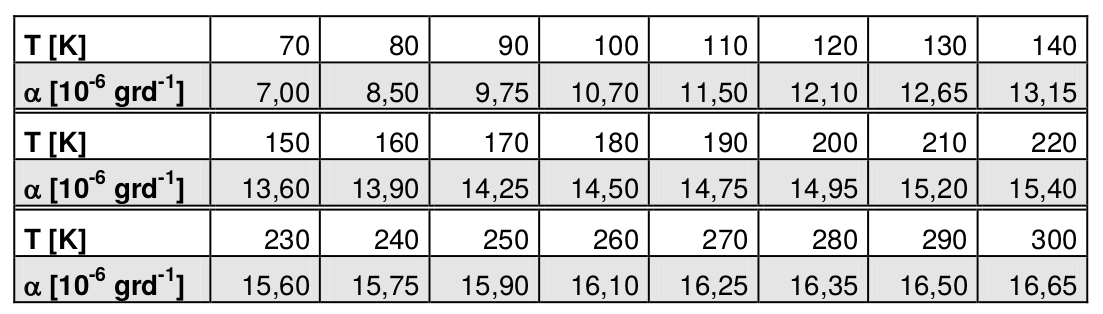
\includegraphics[scale=1.0]{bilder/alpha.pdf}
	\caption{Darstellung der berechneten Dämpfungen des langen \CU-Kabels.}
\label{fig:bilder/alpha}
\end{figure}

%%%%%%%%%%%%%%%%%%%%%%%%%%%%%%%%%%%%%%%%%%%%%%%%%%%%%%%%%%%%%%%%%%%%%%%%%%%
%                 Spannungsverlauf offen kurzgeschlossen                  %
%%%%%%%%%%%%%%%%%%%%%%%%%%%%%%%%%%%%%%%%%%%%%%%%%%%%%%%%%%%%%%%%%%%%%%%%%%%

\clearpage
\subsection{Spannungsverlauf bei offenen und kurzgeschlossenem Ende}
\label{sub:spannungsverlauf_bei_offenen_und_kurzgeschlossenem_ende}

% ==================================================
% 	Kabellänge aus Laufzeitmessung
% ==================================================

\subsubsection{Bestimmung der Kabellänge durch Laufzeitmessung}
\label{ssub:bestimmung_der_kabell_nge_durch_laufzeitmessung}

Hier wird die Länge der drei Kabel durch Betrachtung der Spannungsverläufe am
Anfang des Kabels bei offenen und kurzgeschlossenem Ende bestimmt. Hieran
lassen sich die Zeiten $t_1$, den Beginn des einlaufenden Impulses, und $t_2$,
den Beginn des reflektierten Impulses, ablesen. Die Länge der Kabel lassen sich
schließlich mit%
\begin{equation}
  l = \frac{v \Delta t}{2}, \qquad \Delta t = t_2 - t_1, \quad \text{und} \quad
  v = \frac{1}{\sqrt{LC}} = \frac{\text{c}}{\sqrt{\epsilon_r}}
  \label{eq:laenge}
\end{equation}
bestimmen, wobei $v$ die Ausbreitungsgeschwindigkeit,
$\text{c}$ die Lichtgeschwindigkeit und $\epsilon_r = 2.25$
die Dielektrizitätskonstante des Dielektrikums ist.
Die aufgenommenen Oszillosgraphenbilder sind in de
Abbildungen~\ref{fig:oszi_50k_offen} bis~\ref{fig:oszi_50l_kurz} dargestellt.
Im Anhang sind diese Bilder mit abgelesenen Zeiten zu finden.
Als Fehler der Zeiten wird die Ablesegenauigkeit in den Bildern
genommen. Die Werte befinden sich in Tabelle~\ref{tab:Zeiten}.
Die hiermit und mit der Gleichungen~\eqref{eq:laenge} berechneten Längen
befinden sich in Tabelle~\ref{tab:Laengen}.

\begin{table}[hb]
  \centering
  \begin{tabular}{lcccc}
    \midrule
    \midrule
    & \multicolumn{2}{c}{offenes Ende} &
    \multicolumn{2}{c}{kurzgeschlossenes Ende} \\
    \cmidrule(lr{0.75em}){2-5}
    % \cline{2-5}
    & $t_1 / \si{\nano\second}$ & $t_2 / \si{\nano\second}$    &
    $t_1 / \si{\nano\second}$ & $t_2 / \si{\nano\second}$ \\
    \midrule
    \CU, kurz         & $104 \pm 5$       & $307 \pm 5$       & $105 \pm 5$       & $307 \pm 5$      \\
\BU               & $105 \pm 5$       & $308 \pm 5$       & $104 \pm 5$       & $306 \pm 5$      \\
\CU, lang         & $530 \pm 50$      & $1400 \pm 50$     & $530 \pm 50$      & $1400 \pm 50$    \\
    \midrule
    \midrule
  \end{tabular}
  \caption{Darstellung der abgelesenen Zeiten $t_1$ und $t_2$ der
  jeweiligen Kabel.}
  \vspace{2em}
  \label{tab:Zeiten}
\end{table}

\begin{table}[h]
  \centering
  \begin{tabular}{lcc}
    \midrule
    \midrule
    & \multicolumn{2}{c}{$l / \si{\meter}$} \\
    \cmidrule(lr{0.75em}){2-3}
    & offenes Ende & kurzgeschlossenes Ende \\
    \midrule
    $\SI{50}{\ohm}$, kurz & 105.0 \pm 5.0     & 308.0 \pm 5.0     & 104.0 \pm 5.0     & 306.0 \pm 5.0    \\
$\SI{75}{\ohm}$, kurz & 104.0 \pm 5.0     & 307.0 \pm 5.0     & 105.0 \pm 5.0     & 307.0 \pm 5.0    \\
$\SI{50}{\ohm}$, lang & 530.0 \pm 50.0    & 1400 \pm 50       & 530.0 \pm 50.0    & 1400 \pm 50      \\
    \midrule
    \midrule
  \end{tabular}
  \caption{Darstellung der berechneten Längen $l$ der jeweiligen Kabel mit
    offenem und kurzgeschlossenem Ende.}
  \label{tab:Laengen}
\end{table}

\begin{figure}[ht]
  \centering
  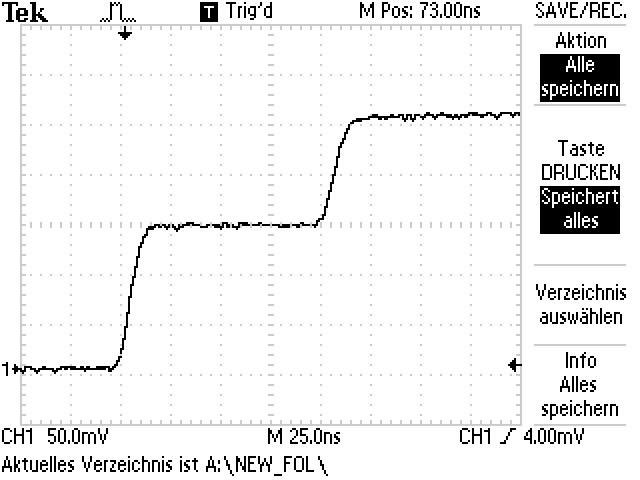
\includegraphics[scale=1.0]{bilder/reflexion/F0000TEK.JPG}
  \caption{Mit dem Oszilloskop aufgenommenes Bild des kurzen \CU-Kabels mit
  offenem Ende.}
  \label{fig:oszi_50k_offen}
  \vspace{2em}
  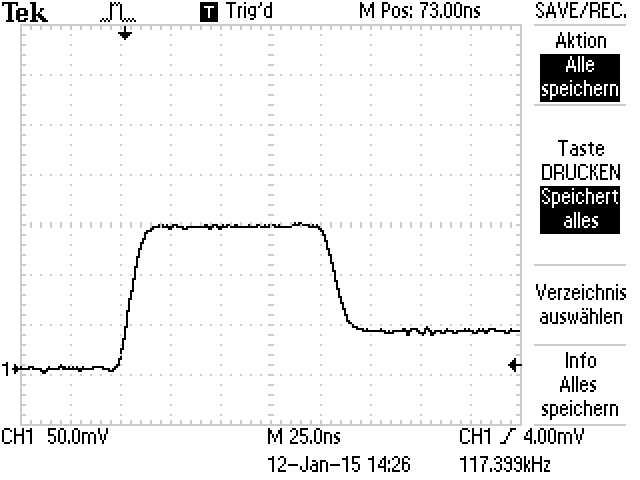
\includegraphics[scale=1.0]{bilder/reflexion/F0001TEK.JPG}
  \caption{Mit dem Oszilloskop aufgenommenes Bild des kurzen \CU-Kabels mit
  kurzgeschlossenem Ende.}
  \label{fig:oszi_50k_kurz}
\end{figure}
\begin{figure}[ht]
  \centering
  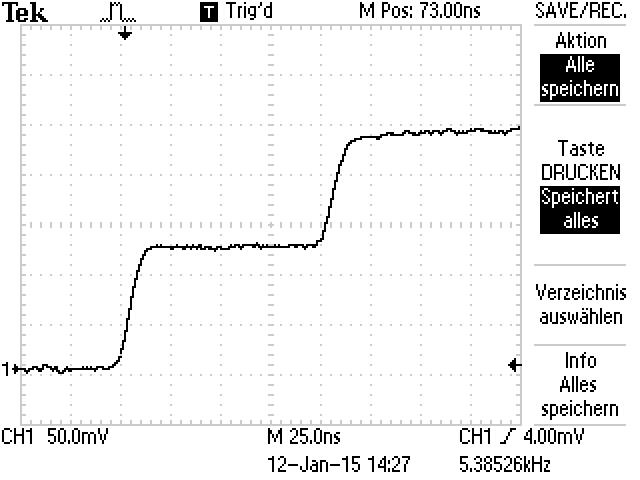
\includegraphics[scale=1.0]{bilder/reflexion/F0002TEK.JPG}
  \caption{Mit dem Oszilloskop aufgenommenes Bild des kurzen \BU-Kabels mit
  offenem Ende.}
  \label{fig:oszi_75k_offen}
  \vspace{2em}
  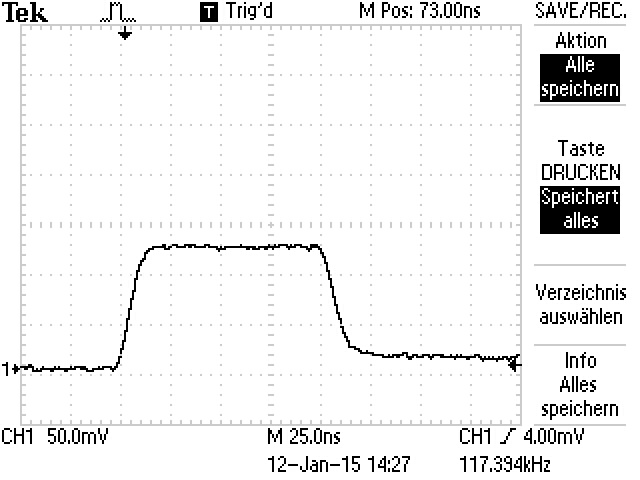
\includegraphics[scale=1.0]{bilder/reflexion/F0003TEK.JPG}
  \caption{Mit dem Oszilloskop aufgenommenes Bild des kurzen \BU-Kabels mit
  kurzgeschlossenem Ende.}
  \label{fig:oszi_75k_kurz}
\end{figure}
\begin{figure}[ht]
  \centering
  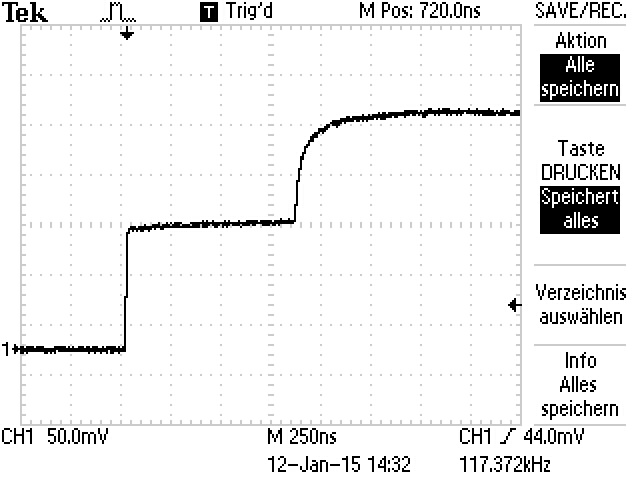
\includegraphics[scale=1.0]{bilder/reflexion/F0004TEK.JPG}
  \caption{Mit dem Oszilloskop aufgenommenes Bild des langen \CU-Kabels mit
  offenem Ende.}
  \label{fig:oszi_50l_offen}
  \vspace{2em}
  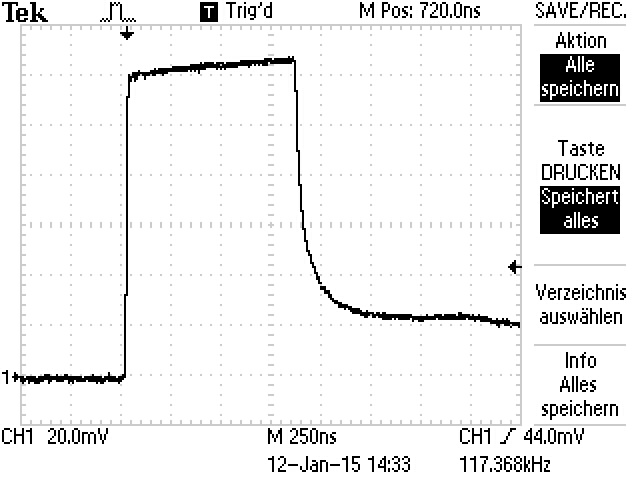
\includegraphics[scale=1.0]{bilder/reflexion/F0005TEK.JPG}
  \caption{Mit dem Oszilloskop aufgenommenes Bild des langen \CU-Kabels mit
  kurzgeschlossenem Ende.}
  \label{fig:oszi_50l_kurz}
\end{figure}

% ==================================================
% 	Leitungskonstanten
% ==================================================

\clearpage
\subsubsection{Bestimmung der Leitungskonstanten}
\label{ssub:bestimmung_der_leitungskonstanten}

In diesem und den folgenden Unterkapiteln werden Daten aus den
Abbildungen~\ref{fig:oszi_50l_offen} und~\ref{fig:oszi_50l_kurz} über den
ganzen $t$-Bereich oder nur bestimmte Teilbereiche mit Hilfe des Programms
\texttt{Engauge} digitalisiert, um eine bessere Auswertung der Daten zu
ermöglichen. Des weiteren ist die Bestimmung der Leitungskonstante nur bei
dem langen \CU-Kabel möglich, da nur hier der kapazitive und induktive Verlauf
der Spannung zu sehen ist. Im Folgenden werden daher nun die Leitungskonstanten
des langen \CU-Kabels bestimmt.

\paragraph{Der Widerstands}
\label{par:der_widerstands}

Hier wird das Oszillosgraphenbild~\ref{fig:oszi_50l_kurz} digitalisiert.
Die erhaltenen Daten befinden sich in Tabelle~\ref{tab:R_Daten} und werden
in Abbildung~\ref{fig:R_Daten} graphisch dargestellt.
Mit Hilfe der Beziehung
\begin{equation}
  U_1 (1 + \Gamma) = U_0 \quad \Rightarrow \quad \Gamma = \frac{U_0}{U_1} - 1
  \label{eq:Gamma_R}
\end{equation}
kann der Reflektionsfaktor $\Gamma$ bestimmt werden. Einsetzen des Ergebnisses
in
\begin{equation}
  \Gamma = \frac{R-Z_0}{R+Z_0} \quad \Rightarrow \quad
  R = - \frac{Z_0(\Gamma + 1)}{\Gamma - 1}
  \label{eq:R}
\end{equation}
liefert schließlich den gewünschten Widerstand $R$.
Hierbei gilt für den Wellenwiderstand $Z_0 = \SI{50}{\ohm}$.
Es gilt also $U_0$ und $U_1$ zu bestimmen, wobei $U_0$ die Höhe des Pulses aus
Abbildung~\ref{fig:R_Daten} ist und $U_1$ die Höhe der Spannung nach Abfall des
Pulses. Um die Spannungen $U_1$ und $U_0$ bestimmen zu können, muss zudem eine
Offsetspannung $U_\text{off}$ ermittelt werden.
Die eben genannten Spannungen werden entsprechend
\begin{align}
  \begin{aligned}
    U_\text{off} &= \overline{U(t)}\,, \\
    U_1          &= \overline{U(t)}\,, \\
    U_0          &= \overline{U(t)}\,,
  \end{aligned}
  \qquad
  \begin{aligned}
    &t~< \SI{500}{\nano\second} \\
    \SI{750}{\nano\second}  <~&t~< \SI{1360}{\nano\second} \\
    \SI{2000}{\nano\second} <~&t~< \SI{2250}{\nano\second}
  \end{aligned}
\end{align}
bestimmt, wobei $U(t)$ und $t$ aus Tabelle~\ref{tab:R_Daten} bzw.
Abbildung~\ref{fig:R_Daten} entnommen werden.
Die so berechneten Werte lauten
\begin{align}
  U_\text{off} &= \SI[parse-numbers = false]{14.96 \pm 0.09}{\volt} \\
  U_0 &= \SI[parse-numbers = false]{24.36 \pm 0.09}{\volt} \\
  U_1 &= \SI[parse-numbers = false]{25.79 \pm 0.14}{\volt}~.
\end{align}
Damit berechnet sich der Widerstand nach Gleichung~\eqref{eq:Gamma_R} und
\eqref{eq:R} zu
\begin{equation}
  \underline{R = $-40.0$           & $19.2$            & $830.0$           & $142.4$           & $1470.0$          & $62.0$           \\
$5.0$             & $18.4$            & $875.0$           & $142.8$           & $1485.0$          & $58.8$           \\
$40.0$            & $18.0$            & $905.0$           & $143.6$           & $1500.0$          & $54.8$           \\
$90.0$            & $17.6$            & $955.0$           & $144.0$           & $1535.0$          & $53.2$           \\
$130.0$           & $19.2$            & $1015.0$          & $144.0$           & $1560.0$          & $50.0$           \\
$170.0$           & $18.8$            & $1055.0$          & $144.0$           & $1595.0$          & $48.0$           \\
$220.0$           & $18.8$            & $1100.0$          & $144.8$           & $1635.0$          & $47.2$           \\
$255.0$           & $18.4$            & $1150.0$          & $144.4$           & $1675.0$          & $45.6$           \\
$295.0$           & $18.4$            & $1195.0$          & $144.8$           & $1720.0$          & $44.4$           \\
$340.0$           & $18.4$            & $1235.0$          & $145.6$           & $1760.0$          & $44.0$           \\
$385.0$           & $18.0$            & $1280.0$          & $145.6$           & $1800.0$          & $43.6$           \\
$425.0$           & $18.8$            & $1330.0$          & $145.6$           & $1850.0$          & $43.2$           \\
$470.0$           & $18.4$            & $1365.0$          & $146.0$           & $1895.0$          & $43.2$           \\
$510.0$           & $19.2$            & $1370.0$          & $142.0$           & $1945.0$          & $43.2$           \\
$515.0$           & $22.8$            & $1375.0$          & $138.4$           & $1980.0$          & $42.8$           \\
$520.0$           & $30.8$            & $1380.0$          & $130.4$           & $2030.0$          & $42.8$           \\
$525.0$           & $38.4$            & $1385.0$          & $118.8$           & $2075.0$          & $43.2$           \\
$530.0$           & $90.4$            & $1390.0$          & $102.8$           & $2120.0$          & $43.2$           \\
$535.0$           & $106.0$           & $1395.0$          & $99.2$            & $2170.0$          & $43.2$           \\
$540.0$           & $122.0$           & $1400.0$          & $95.2$            & $2215.0$          & $43.2$           \\
$550.0$           & $137.6$           & $1405.0$          & $87.6$            & $2260.0$          & $42.8$           \\
$570.0$           & $139.2$           & $1410.0$          & $83.6$            & $2300.0$          & $42.8$           \\
$605.0$           & $140.8$           & $1415.0$          & $80.0$            & $2345.0$          & $42.0$           \\
$645.0$           & $140.4$           & $1420.0$          & $76.0$            & $2390.0$          & $40.8$           \\
$685.0$           & $141.2$           & $1430.0$          & $72.4$            & $2420.0$          & $40.8$           \\
$730.0$           & $141.6$           & $1440.0$          & $68.8$            & -                 & -                \\
$780.0$           & $142.4$           & $1455.0$          & $65.6$            & -                 & -                \\}~.
\end{equation}

% Tabellen und Bilder
\begin{table}[hb]
  \centering
  \begin{tabular}{cc|cc|cc}
    \midrule
    \midrule
    $t / \si{\nano\second}$ & $U / \si{\milli\volt}$ &
    $t / \si{\nano\second}$ & $U / \si{\milli\volt}$ &
    $t / \si{\nano\second}$ & $U / \si{\milli\volt}$ \\
    \midrule
    $-40.0$           & $19.2$            & $830.0$           & $142.4$           & $1470.0$          & $62.0$           \\
$5.0$             & $18.4$            & $875.0$           & $142.8$           & $1485.0$          & $58.8$           \\
$40.0$            & $18.0$            & $905.0$           & $143.6$           & $1500.0$          & $54.8$           \\
$90.0$            & $17.6$            & $955.0$           & $144.0$           & $1535.0$          & $53.2$           \\
$130.0$           & $19.2$            & $1015.0$          & $144.0$           & $1560.0$          & $50.0$           \\
$170.0$           & $18.8$            & $1055.0$          & $144.0$           & $1595.0$          & $48.0$           \\
$220.0$           & $18.8$            & $1100.0$          & $144.8$           & $1635.0$          & $47.2$           \\
$255.0$           & $18.4$            & $1150.0$          & $144.4$           & $1675.0$          & $45.6$           \\
$295.0$           & $18.4$            & $1195.0$          & $144.8$           & $1720.0$          & $44.4$           \\
$340.0$           & $18.4$            & $1235.0$          & $145.6$           & $1760.0$          & $44.0$           \\
$385.0$           & $18.0$            & $1280.0$          & $145.6$           & $1800.0$          & $43.6$           \\
$425.0$           & $18.8$            & $1330.0$          & $145.6$           & $1850.0$          & $43.2$           \\
$470.0$           & $18.4$            & $1365.0$          & $146.0$           & $1895.0$          & $43.2$           \\
$510.0$           & $19.2$            & $1370.0$          & $142.0$           & $1945.0$          & $43.2$           \\
$515.0$           & $22.8$            & $1375.0$          & $138.4$           & $1980.0$          & $42.8$           \\
$520.0$           & $30.8$            & $1380.0$          & $130.4$           & $2030.0$          & $42.8$           \\
$525.0$           & $38.4$            & $1385.0$          & $118.8$           & $2075.0$          & $43.2$           \\
$530.0$           & $90.4$            & $1390.0$          & $102.8$           & $2120.0$          & $43.2$           \\
$535.0$           & $106.0$           & $1395.0$          & $99.2$            & $2170.0$          & $43.2$           \\
$540.0$           & $122.0$           & $1400.0$          & $95.2$            & $2215.0$          & $43.2$           \\
$550.0$           & $137.6$           & $1405.0$          & $87.6$            & $2260.0$          & $42.8$           \\
$570.0$           & $139.2$           & $1410.0$          & $83.6$            & $2300.0$          & $42.8$           \\
$605.0$           & $140.8$           & $1415.0$          & $80.0$            & $2345.0$          & $42.0$           \\
$645.0$           & $140.4$           & $1420.0$          & $76.0$            & $2390.0$          & $40.8$           \\
$685.0$           & $141.2$           & $1430.0$          & $72.4$            & $2420.0$          & $40.8$           \\
$730.0$           & $141.6$           & $1440.0$          & $68.8$            & -                 & -                \\
$780.0$           & $142.4$           & $1455.0$          & $65.6$            & -                 & -                \\
    \midrule
    \midrule
  \end{tabular}
  \caption{Datstellung der digitalisierten Daten des
    Oszillosgraphenbild~\ref{fig:oszi_50l_kurz}.}
  \label{tab:R_Daten}
\end{table}
\begin{figure}[hb]
  \centering
  \includegraphics[scale=1.0]{bilder/R.pdf}
  \caption{Graphische Darstellung der digitalisierten Daten des
    Oszillosgraphenbild~\ref{fig:oszi_50l_kurz}.}
\label{fig:R_Daten}
\end{figure}

\clearpage
\paragraph{Die Induktivität}
\label{par:die_induktivitaet}

Ein kurzgeschlossenes Koaxialkabel zeigt ein rein induktives Verhalten, daher
wird zur Bestimmung der Induktivität ebenfalls das
Oszillosgraphenbild~\ref{fig:oszi_50l_kurz} mit den entsprechend
digitalisierten Daten aus Tabelle~\ref{tab:R_Daten} verwandt.
Jedoch werden diese Daten auf den für die Induktivität relevanten Teil
eingeschränkt, sodass nur die Werte $U(t)$ aus
\begin{equation}
  \SI{1430}{\nano\second} <~t~< \SI{2250}{\nano\second}
\end{equation}
betrachtet werden. Diese Werte sind in Abbildung~\ref{fig:induktivitaetsbelag}
graphisch dargestellt.
Die Abfallende Flanke des Pulses entspricht nun einem Ausschaltvorgang
einer Spule entsprechend
\begin{equation}
  U(t) = U_0 \exp(-\frac{t}{\tau}) + U_\text{off} \quad \text{mit} \quad
  \tau = \frac{L}{R+Z_0}~,
  \label{eq:L_abschalt}
\end{equation}
wobei $R$ den oben bestimmten Widerstand und $U_\text{off}$ die
Offsetspannung zu \SI{0}{\volt} darstellt. Durch Umstellen und Logarithmierung
der Gleichung \eqref{eq:L_abschalt} ergibt sich eine Geradengleichung der Form
\begin{equation}
  \ln(U - U_\text{off}) = -\frac{t}{\tau} + \ln U_0 \coloneqq
  m \cdot t + \ln U_0 \quad \text{mit} \quad m = - \frac{1}{\tau}
\end{equation}
womit schließlich eine lineare Regression durchgeführt und aus der
Steigung der Induktivität bestimmt werden kann.
Die Offsetspannung wird entsprechend%
\begin{equation}
  U_\text{off} = \overline{U(t)}\,,
  \quad \SI{2100}{\nano\second} <~t~< \SI{2250}{\nano\second}
\end{equation}
zu%
\begin{equation}
  U_\text{off} = \SI{64.11}{\milli\volt}
\end{equation}
bestimmt.
In Abbildung~\ref{fig:induktivitaetsbelag_fit} sind nun die Daten
${\ln(U - U_\text{off})}$ sowie die dazugehörige lineare Regression eingetragen.
Die entsprechenden Daten befinden sich in Tabelle~\ref{tab:L_Daten}.
Der Fit ergibt dabei die Gleichung
\begin{equation}
  \sisetup{per-mode=reciprocal-positive-first}
  G_L(t) = \SI[parse-numbers = false]{-0.0053 \pm 0.0004}{\per\nano\second}\, \cdot \,t\, + \SI[parse-numbers = false]{11.6 \pm 0.7}{}~.
  \label{eq:L_fit}
\end{equation}
Aus der Steigung von~\ref{eq:L_fit} wird nun mit Gleichung~\eqref{eq:L_abschalt} der
Induktivität zu
\begin{equation}
  \underline{L = \SI[parse-numbers = false]{226.0 \pm 4.2}{\milli\henry}}
  \label{eq:indukivitaetsbelag}
\end{equation}
bestimmt.

\begin{table}[htpb]
  \centering
  \begin{tabular}{cccc}
    \midrule
    \midrule
    $t / \si{\nano\second}$ & $U / \si{\milli\volt}$ &
    $U - U_\text{off} / \si{\milli\volt}$ & $\ln(U - U_\text{off})$ \\
    \midrule
    \SI[parse-numbers = false]{226.0 \pm 4.2}{\milli\henry}
    \midrule
    \midrule
  \end{tabular}
  \caption{Darstellung der für die Induktivität relevanten Daten sowie
  die berechneten Werte für den Fit.}
  \label{tab:L_Daten}
\end{table}
\begin{figure}[htpb]
  \centering
  \includegraphics[scale=1.0]{bilder/L.pdf}
  \caption{Darstellung der für die zur Bestimmung der Induktivität
    relevanten digitalisierten Daten von Abbildung~\ref{fig:oszi_50l_kurz}.}
  \label{fig:induktivitaetsbelag}
  \includegraphics[scale=1.0]{bilder/L_fit.pdf}
  \caption{Darstellung der für die zur Bestimmung der Induktivität
    relevanten digitalisierten Daten von Abbildung~\ref{fig:oszi_50l_kurz}.}
  \label{fig:induktivitaetsbelag_fit}
\end{figure}

\clearpage
\paragraph{Die Kapazität}
\label{par:die_kapazitaet}

Entgegen der Induktivität zeigt ein Koaxialkabel mit offenem Ende ein
rein kapazitives Verhalten. Somit wird zur Bestimmung der Kapazität das
Oszillosgraphenbild~\ref{fig:oszi_50l_offen} verwandt. Die entsprechenden
digitalisierten Daten sind in Tabelle~\ref{tab:C_roh_Daten} und
Abbildung~\ref{fig:C_roh_Daten} dargestellt.
Die Einschränkung der relevanten Daten bezieht sich hier auf $U(t)$ aus
\begin{equation}
  \quad \SI{1370}{\nano\second} <~t~< \SI{1650}{\nano\second}~.
\end{equation}
Den zu betrachtenden Verlauf entspricht hier einer Aufladekurve eines
Kondensators gemäß
\begin{equation}
  U = U_0\qty(1 - \exp(-\frac{t}{\tau})) \quad \text{mit} \quad
  \tau = RC~,
  \label{eq:Aufladekurve_C}
\end{equation}
wobei $R$ wiederum der obige Widerstand ist. Diese Gleichung kann wieder
linearisiert werden zu
\begin{equation}
  \ln(U_0 - U) = - \frac{t}{\tau} + \ln(U_0)~,
  \label{eq:C_lin}
\end{equation}
woraus aus der Steigung die Kapazität bestimmt werden kann.
Die Sättigungsspannung $U_0$ wird dabei entsprechend
\begin{equation}
  U_0 = \overline{U(t)}\,,
  \quad \SI{2000}{\nano\second} <~t
\end{equation}
zu
\begin{equation}
  U_0 = \SI{311.78}{\milli\volt}
\end{equation}
bestimmt. Die für den Fit relevanten Daten sind in Tabelle~\ref{tab:C_fit}
dargestellt. Der Fit befindet sich in Abbildung~\ref{fig:C_fit}.
Die aus dem Fit erhaltene Gleichung lautet
\begin{equation}
  \sisetup{per-mode=reciprocal-positive-first}
  1375\phantom{.}   & 215.910           & 95.869            & 4.563            \\
1380\phantom{.}   & 225.883           & 85.896            & 4.453            \\
1385\phantom{.}   & 234.859           & 76.920            & 4.343            \\
1390\phantom{.}   & 244.832           & 66.947            & 4.204            \\
1395\phantom{.}   & 253.807           & 57.972            & 4.060            \\
1405\phantom{.}   & 262.781           & 48.998            & 3.892            \\
1420\phantom{.}   & 271.753           & 40.026            & 3.690            \\
1435\phantom{.}   & 279.727           & 32.052            & 3.467            \\
1465\phantom{.}   & 286.697           & 25.082            & 3.222            \\
1490\phantom{.}   & 292.672           & 19.107            & 2.950            \\
1525\phantom{.}   & 296.648           & 15.131            & 2.717            \\
1560\phantom{.}   & 301.622           & 10.157            & 2.318            \\
1600\phantom{.}   & 303.601           & \phantom{0}8.178  & 2.101            \\
1645\phantom{.}   & 305.578           & \phantom{0}6.201  & 1.825            \\~.
  \label{eq:C_fit}
\end{equation}
Aus der Steigung kann nun die Kapazität mit Hilfe von
Gleichung~\eqref{eq:Aufladekurve_C} zu
\begin{equation}
  \underline{C = \SI[parse-numbers = false]{1.82 \pm 0.16}{\nano\farad}}
\end{equation}
bestimmt werden.

% Tabellen und Plots
\begin{table}[htpb]
  \centering
  \begin{tabular}{cc|cc|cc}
    \midrule
    \midrule
    $t / \si{\nano\second}$ & $U / \si{\milli\volt}$ &
    $t / \si{\nano\second}$ & $U / \si{\milli\volt}$ &
    $t / \si{\nano\second}$ & $U / \si{\milli\volt}$ \\
    \midrule
    --40\phantom{.}   & \phantom{0}76.824 & \phantom{0}865\phantom{.} & 200.154           & 1560\phantom{.}   & 301.622          \\
\phantom{0}10\phantom{.} & \phantom{0}75.806 & \phantom{0}910\phantom{.} & 201.133           & 1600\phantom{.}   & 303.601          \\
\phantom{0}60\phantom{.} & \phantom{0}76.784 & \phantom{0}955\phantom{.} & 202.113           & 1645\phantom{.}   & 305.578          \\
105\phantom{.}    & \phantom{0}76.766 & \phantom{0}995\phantom{.} & 201.099           & 1690\phantom{.}   & 305.560          \\
150\phantom{.}    & \phantom{0}75.751 & 1030\phantom{.}   & 200.088           & 1735\phantom{.}   & 305.542          \\
190\phantom{.}    & \phantom{0}77.730 & 1070\phantom{.}   & 201.069           & 1775\phantom{.}   & 308.519          \\
235\phantom{.}    & \phantom{0}75.717 & 1115\phantom{.}   & 201.051           & 1815\phantom{.}   & 308.503          \\
285\phantom{.}    & \phantom{0}75.697 & 1160\phantom{.}   & 202.031           & 1860\phantom{.}   & 310.480          \\
330\phantom{.}    & \phantom{0}75.679 & 1210\phantom{.}   & 203.008           & 1910\phantom{.}   & 310.460          \\
375\phantom{.}    & \phantom{0}75.661 & 1255\phantom{.}   & 202.991           & 1955\phantom{.}   & 312.437          \\
415\phantom{.}    & \phantom{0}76.642 & 1295\phantom{.}   & 201.977           & 1995\phantom{.}   & 310.426          \\
455\phantom{.}    & \phantom{0}75.629 & 1340\phantom{.}   & 202.957           & 2030\phantom{.}   & 311.409          \\
500\phantom{.}    & \phantom{0}75.611 & 1365\phantom{.}   & 206.937           & 2070\phantom{.}   & 311.394          \\
515\phantom{.}    & \phantom{0}83.585 & 1375\phantom{.}   & 215.910           & 2120\phantom{.}   & 313.369          \\
520\phantom{.}    & \phantom{0}93.558 & 1380\phantom{.}   & 225.883           & 2160\phantom{.}   & 311.358          \\
525\phantom{.}    & 112.509           & 1385\phantom{.}   & 234.859           & 2200\phantom{.}   & 312.339          \\
530\phantom{.}    & 142.432           & 1390\phantom{.}   & 244.832           & 2240\phantom{.}   & 313.321          \\
535\phantom{.}    & 161.383           & 1395\phantom{.}   & 253.807           & 2280\phantom{.}   & 313.305          \\
540\phantom{.}    & 181.331           & 1405\phantom{.}   & 262.781           & 2325\phantom{.}   & 311.292          \\
565\phantom{.}    & 196.283           & 1420\phantom{.}   & 271.753           & 2370\phantom{.}   & 310.276          \\
600\phantom{.}    & 197.267           & 1435\phantom{.}   & 279.727           & 2405\phantom{.}   & 311.260          \\
640\phantom{.}    & 196.253           & 1465\phantom{.}   & 286.697           & 2450\phantom{.}   & 310.244          \\
680\phantom{.}    & 199.230           & 1490\phantom{.}   & 292.672           & -                 & -                \\
720\phantom{.}    & 199.214           & 1525\phantom{.}   & 296.648           & -                 & -                \\
    \midrule
    \midrule
  \end{tabular}
  \caption{Darstellung der digitalisierten Daten aus dem
    Oszillosgraphenbild~\ref{fig:oszi_50l_offen}.}
\label{tab:C_roh_Daten}
\end{table}

\begin{table}[htpb]
  \centering
  \begin{tabular}{cccc}
    \midrule
    \midrule
    $t / \si{\nano\second}$ & $U / \si{\milli\volt}$ &
    $U_0 - U / \si{\milli\volt}$ & $\ln(U_0 - U) / \si{\milli\volt}$ \\
    \midrule
    1375\phantom{.}   & 215.910           & 95.869            & 4.563            \\
1380\phantom{.}   & 225.883           & 85.896            & 4.453            \\
1385\phantom{.}   & 234.859           & 76.920            & 4.343            \\
1390\phantom{.}   & 244.832           & 66.947            & 4.204            \\
1395\phantom{.}   & 253.807           & 57.972            & 4.060            \\
1405\phantom{.}   & 262.781           & 48.998            & 3.892            \\
1420\phantom{.}   & 271.753           & 40.026            & 3.690            \\
1435\phantom{.}   & 279.727           & 32.052            & 3.467            \\
1465\phantom{.}   & 286.697           & 25.082            & 3.222            \\
1490\phantom{.}   & 292.672           & 19.107            & 2.950            \\
1525\phantom{.}   & 296.648           & 15.131            & 2.717            \\
1560\phantom{.}   & 301.622           & 10.157            & 2.318            \\
1600\phantom{.}   & 303.601           & \phantom{0}8.178  & 2.101            \\
1645\phantom{.}   & 305.578           & \phantom{0}6.201  & 1.825            \\
    \midrule
    \midrule
  \end{tabular}
  \caption{Darstellung der für den Fit relevanten Daten.}
\label{tab:C_fit}
\end{table}

\begin{figure}[htpb]
  \centering
  \includegraphics[scale=1.0]{bilder/C.pdf}
  \caption{Graphische Darstellung der digitalisierten Daten des langen
    \CU-Kabels mit offenem Ende.}
\label{fig:C_roh_Daten}
  \includegraphics[scale=1.0]{bilder/C_fit.pdf}
  \caption{Graphische Darstellung der digitalisierten Daten des langen
    \CU-Kabels mit offenem Ende.}
\label{fig:C_fit}
\end{figure}

% ==================================================
% 	Schmitt-Diagramm
% ==================================================

\clearpage
\subsubsection{Bestimmung der Kabellänge über ein Smith-Diagramm}
\label{ssub:bestimmung_der_kabell_nge_ber_ein_smith_diagramm}

Nun soll die Länge des langen \BU-Kabels (die Leitungskonstanten der anderen
Kabel konnten wie oben beschrieben nicht bestimmt werden) mit Hilfe eines
Smith-Diagramms bestimmt werden. Das verwandte Smith-Diagramm ist
im Anhang zu finden. Die vollständige Umdrehung der
Smith-Diagramms entspricht einer halben Wellenlänge $\lambda$, sodass die Länge
des Kabels durch
\begin{equation}
  l = \frac{\lambda}{2} \cdot \frac{\varphi}{2 \pi}
\end{equation}
angegeben werden kann, wobei $\varphi$ die Phasenverschiebung nach der Reflexion
am Kabelende beschreibt. Die Wellenlänge lässt sich zudem durch
\begin{equation}
  \lambda = \frac{c}{f \sqrt{\epsilon_r}}
\end{equation}
ausdrücken.
Das heißt, gesucht ist zunächst die Phasenverschiebung $\varphi$.
Dazu wird nun der kurzgeschlossene Fall betrachtet.
Die Impedanz des Kabels beträgt hier
\begin{equation}
  Z_L = R + \text{i}\, 2 \pi f L~,
\end{equation}
wobei $R$ und $L$ die oben bestimmten Widerstands- bzw. Induktivitätsbeläge
sind. Somit ergibt sich die Impedanz zu
\begin{equation}
  Z_L = \SI{(8.71 + 0.06i)}{\ohm}~.
\end{equation}
Die Phasenverschiebung $\varphi$ kann nun beschrieben werden als Winkel
zwischen den Reflexionsfaktoren
\begin{equation}
  \Gamma_{L,R} = \frac{Z - Z_0}{Z + Z_0}\,, \quad Z = R, Z_L~,
  % -0.70 + 0.00i
\end{equation}
wobei
\begin{equation}
  \Gamma_R = \SI[parse-numbers = false]{-0.7009 \pm 0.0025}{}~,
\end{equation}
der Reflektionsfaktor am Ende des Kabels,
aus Gleichung \eqref{eq:Gamma_R} gegeben ist.
Damit kann nun die Phase mit
\begin{equation}
  \varphi = \measuredangle(\Gamma_L, \Gamma_R)
\end{equation}
berechnet werden, womit sich schließlich für die Länge
\begin{equation}
  l_L = \underline{\SI{32.0}{\meter}}
\end{equation}
ergibt.
Im offenen Fall gilt
\begin{align}
  \Gamma_R &= 1 \\
  Z_L &= - \frac{i}{2\pi\ fC}~.
\end{align}
Hiermit wird die analog zum kurzgeschlossenen Fall die Länge zu
\begin{equation}
  L_C = \SI{19.8}{\meter}
\end{equation}
bestimmt.

% ==================================================
% 	Mehrfachreflexion
% ==================================================

\subsection{Mehrfachreflexion}
\label{sub:mehrfachreflexion}

In diesem Teil sollen Reflexionen betrachtet werden, die entstehen, wenn zwei
Kabel mit unterschiedlichem Widerstand hintereinandergeschaltet werden.
In diesem Fall das kurze \CU und das kurze \BU-Kabel.
Das aufgenommene Oszillosgraphenbild und die entsprechend digitalisierten Werte
sind in Abbildung~\ref{fig:mehrfachreflexion_roh}
bzw.~\ref{fig:mehrfachreflexion} dargestellt.
Nun werden wieder die Werte der Spannungsplateaus gemittelt, um die
Spannungsflanken und schließlich die Reflexionsfaktoren zu bestimmen.
Die hier verwandten Werte ergeben sich aus
\begin{align*}
  \begin{aligned}
    U_\text{off} &= \overline{U(t)}\,, \\
    U_0          &= \overline{U(t)}\,, \\
    U_1          &= \overline{U(t)}\,, \\
    U_2          &= \overline{U(t)}\,, \\
    U_3          &= \overline{U(t)}\,,
  \end{aligned}
  \qquad
  \begin{aligned}
    &t~< \SI{80}{\nano\second} \\
    \SI{110}{\nano\second} <~&t~< \SI{180}{\nano\second} \\
    \SI{210}{\nano\second}  <~&t~< \SI{285}{\nano\second} \\
    \SI{322}{\nano\second} <~&t~< \SI{380}{\nano\second} \\
    \SI{432}{\nano\second} <~&t
  \end{aligned}
\end{align*}
mit den Ergebnissen
\begin{align*}
  U_\text{off} &= \SI[parse-numbers = false]{202.0 \pm 0.8}{\milli\volt} \\
  U_0 &= \SI[parse-numbers = false]{202.0 \pm 0.8}{\milli\volt} \\
  U_1 &= \SI[parse-numbers = false]{224.5 \pm 1.0}{\milli\volt} \\
  U_2 &= \SI[parse-numbers = false]{330.4 \pm 1.7}{\milli\volt} \\
  U_3 &= \SI[parse-numbers = false]{330.4 \pm 1.7}{\milli\volt}~.
\end{align*}
Von diesen Spannungen wird die Offset-Spannung abgezogen und die folgenden
Spannungsdifferenzen berechnet.
\begin{align*}
  \Delta U_1 &= U_1 - U_0 \\
  \Delta U_2 &= U_2 - U_1 \\
  \Delta U_3 &= U_3 - U_2~.
\end{align*}
Hiermit lassen sich nun die Reflexionsfaktoren zu
\begin{align*}
  \Gamma_L &= \frac{\Delta U_1}{U_0} = \SI[parse-numbers = false]{0.183 \pm 0.012}{} \\
  \Gamma_E &= \frac{\Delta U_3}{\Delta U_2} +
  \frac{\Delta U_2}{U_0(1 - \Gamma_L)}
  = \SI[parse-numbers = false]{0.916 \pm 0.023}{} \\
  \Gamma_R &= \frac{\Delta U_3}{\Delta U_2 \Gamma_E}
  = \SI[parse-numbers = false]{-0.152 \pm 0.019}{}
\end{align*}
bestimmen.
Die Reflexionsfaktoren $\Gamma_L$ und $\Gamma_R$ sollten nach der Theorie
betragsmäßig ca. 0.2 sein. Somit ist anzunehmen, dass die verwandten Kabel von
ihrer Nennimpedanz abweichen.

\begin{figure}[htpb]
  \centering
  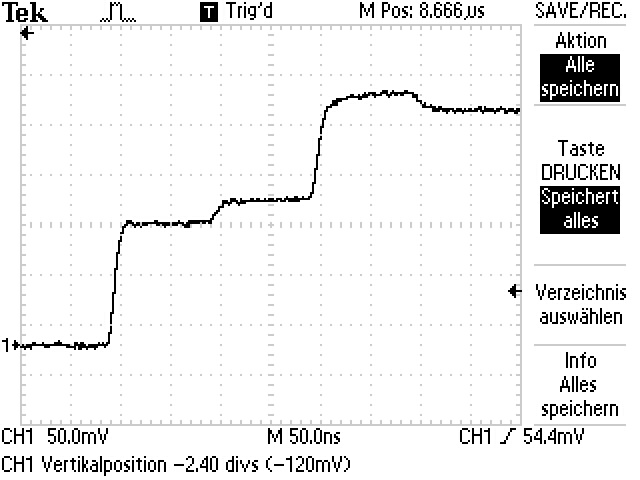
\includegraphics[scale=1.0]{bilder/mehrfachreflexion/F0000TEK.JPG}
  \caption{Aufgenommenes Oszillosgraphenbild bei hintereinandergeschalteten
    \CU- und \BU-Kabel.}
\label{fig:mehrfachreflexion_roh}
  \includegraphics[scale=1.0]{bilder/mehrfachreflexion/mf.pdf}
  \caption{Darstellung der digitalisierten Daten aus dem
    Oszilloskopenbild aus Abbildung~\ref{fig:mehrfachreflexion_roh}}
\label{fig:mehrfachreflexion}
\end{figure}

\subsection{Spannungsverlauf bei drei verschiedenen Abschlusswiderständen}
\label{sub:spannungsverlauf_bei_drei_verschiedenen_abschlusswiderst_nden}

In diesem Versuchsteil sollen die Spannungsverläufe mit drei unterschiedlichen,
noch unbekannten, Abschlusswiderständen untersucht werden.
Hierbei wird das kurze \CU-Kabel verwandt.

\paragraph{Abschluss 1}
\label{ssub:abschluss_1}

Der Spannungsverlauf ist in Abbildung~\ref{fig:abschluss_1} dargestellt.
Im Vergleich der im Anhang befindlichen Abbildung~\ref{fig:abschluesse} handelt
es sich hier um Abschluss, welcher aus einer Reihenschaltung von einem
Widerstand mit einem Kondensator besteht.
Zur Bestimmung des Widerstandes wird so vorgegangen wie in
Abschnitt~\ref{ssub:bestimmung_der_leitungskonstanten}.
Der Widerstand berechnet sich dabei entsprechend \eqref{eq:R}, wobei der
Reflexionsfaktor sich aus den Spannungen $U_0$ und $U_1$ zusammensetzt, welche
nach
\begin{align}
  \begin{aligned}
    U_\text{off} &= \overline{U(t)}\,, \\
    U_1          &= \overline{U(t)}\,, \\
    U_0          &= \SI[parse-numbers = false]{24.36 \pm 0.09}{\volt}
  \end{aligned}
  \qquad
  \begin{aligned}
    &t~< \SI{200}{\nano\second} \\
    \SI{223}{\nano\second}  <~&t~< \SI{302}{\nano\second} \\
    &
  \end{aligned}
\end{align}
bestimmt werden. Die Spannung $U_0$ kann schlecht abgelesen werden, weshalb
dementsprechend ein großer Fehler angenommen wird.
Die Daten sind in Abbildung~\ref{fig:abschluss_1_digitalisiert} dargestellt
sowie in Tabelle~\ref{tab:daten_abschluss_1}.
Die berechneten Werte für $U_0$ und $U_1$ lauten nach Mittelung
\begin{align}
  U_\text{off} &= \SI[parse-numbers = false]{14.96 \pm 0.09}{\volt} \\
  U_1 &= \SI[parse-numbers = false]{25.79 \pm 0.14}{\volt}~.
\end{align}
Damit ergibt sich der Widerstand zu
\begin{equation}
  \underline{R = $-40.0$           & $19.2$            & $830.0$           & $142.4$           & $1470.0$          & $62.0$           \\
$5.0$             & $18.4$            & $875.0$           & $142.8$           & $1485.0$          & $58.8$           \\
$40.0$            & $18.0$            & $905.0$           & $143.6$           & $1500.0$          & $54.8$           \\
$90.0$            & $17.6$            & $955.0$           & $144.0$           & $1535.0$          & $53.2$           \\
$130.0$           & $19.2$            & $1015.0$          & $144.0$           & $1560.0$          & $50.0$           \\
$170.0$           & $18.8$            & $1055.0$          & $144.0$           & $1595.0$          & $48.0$           \\
$220.0$           & $18.8$            & $1100.0$          & $144.8$           & $1635.0$          & $47.2$           \\
$255.0$           & $18.4$            & $1150.0$          & $144.4$           & $1675.0$          & $45.6$           \\
$295.0$           & $18.4$            & $1195.0$          & $144.8$           & $1720.0$          & $44.4$           \\
$340.0$           & $18.4$            & $1235.0$          & $145.6$           & $1760.0$          & $44.0$           \\
$385.0$           & $18.0$            & $1280.0$          & $145.6$           & $1800.0$          & $43.6$           \\
$425.0$           & $18.8$            & $1330.0$          & $145.6$           & $1850.0$          & $43.2$           \\
$470.0$           & $18.4$            & $1365.0$          & $146.0$           & $1895.0$          & $43.2$           \\
$510.0$           & $19.2$            & $1370.0$          & $142.0$           & $1945.0$          & $43.2$           \\
$515.0$           & $22.8$            & $1375.0$          & $138.4$           & $1980.0$          & $42.8$           \\
$520.0$           & $30.8$            & $1380.0$          & $130.4$           & $2030.0$          & $42.8$           \\
$525.0$           & $38.4$            & $1385.0$          & $118.8$           & $2075.0$          & $43.2$           \\
$530.0$           & $90.4$            & $1390.0$          & $102.8$           & $2120.0$          & $43.2$           \\
$535.0$           & $106.0$           & $1395.0$          & $99.2$            & $2170.0$          & $43.2$           \\
$540.0$           & $122.0$           & $1400.0$          & $95.2$            & $2215.0$          & $43.2$           \\
$550.0$           & $137.6$           & $1405.0$          & $87.6$            & $2260.0$          & $42.8$           \\
$570.0$           & $139.2$           & $1410.0$          & $83.6$            & $2300.0$          & $42.8$           \\
$605.0$           & $140.8$           & $1415.0$          & $80.0$            & $2345.0$          & $42.0$           \\
$645.0$           & $140.4$           & $1420.0$          & $76.0$            & $2390.0$          & $40.8$           \\
$685.0$           & $141.2$           & $1430.0$          & $72.4$            & $2420.0$          & $40.8$           \\
$730.0$           & $141.6$           & $1440.0$          & $68.8$            & -                 & -                \\
$780.0$           & $142.4$           & $1455.0$          & $65.6$            & -                 & -                \\}~.
\end{equation}
Bei der Bestimmung der Kapazität wird ebenfalls wie in
Abschnitt~\ref{ssub:bestimmung_der_leitungskonstanten} vorgegangen.
Die relevanten Daten für den Fit werden dabei aus dem Bereich
\begin{equation}
  \SI{319}{\nano\second} < t < \SI{600}{\nano\second}
\end{equation}
genommen, während die Sättigungsspannung aus
\begin{equation}
  U_0 = \overline{U(t)}\,,\quad
  \SI{1500}{\nano\second} < t < \SI{2000}{\nano\second}
\end{equation}
bestimmt wird.
Für den Fit wird die Linearisierung \eqref{eq:C_lin} verwandt mit dem
Unterschied, dass die Zeitkonstante und die Kapazität hier durch
\begin{equation}
  \tau = (R + Z_0) C\,,\quad C = - \frac{1}{m (R + Z_0)}
\end{equation}
gegeben ist.
Das Ergebnis des Fits ist in Abbildung~\ref{fig:abschluss_1_fit} dargestellt.
Die erhaltenen Gleichung lautet
\begin{equation}
  1375\phantom{.}   & 215.910           & 95.869            & 4.563            \\
1380\phantom{.}   & 225.883           & 85.896            & 4.453            \\
1385\phantom{.}   & 234.859           & 76.920            & 4.343            \\
1390\phantom{.}   & 244.832           & 66.947            & 4.204            \\
1395\phantom{.}   & 253.807           & 57.972            & 4.060            \\
1405\phantom{.}   & 262.781           & 48.998            & 3.892            \\
1420\phantom{.}   & 271.753           & 40.026            & 3.690            \\
1435\phantom{.}   & 279.727           & 32.052            & 3.467            \\
1465\phantom{.}   & 286.697           & 25.082            & 3.222            \\
1490\phantom{.}   & 292.672           & 19.107            & 2.950            \\
1525\phantom{.}   & 296.648           & 15.131            & 2.717            \\
1560\phantom{.}   & 301.622           & 10.157            & 2.318            \\
1600\phantom{.}   & 303.601           & \phantom{0}8.178  & 2.101            \\
1645\phantom{.}   & 305.578           & \phantom{0}6.201  & 1.825            \\~,
\end{equation}
woraus sich die Kapazität zu
\begin{equation}
  \underline{C = \SI[parse-numbers = false]{1.82 \pm 0.16}{\nano\farad}}
\end{equation}
ergibt.

\begin{table}[htpb]
  \centering
  \begin{tabular}{cc|cc|cc|cc}
    \midrule
    \midrule
    $t/\si{\nano\second}$ & $U/\si{\volt}$ &
    $t/\si{\nano\second}$ & $U/\si{\volt}$ &
    $t/\si{\nano\second}$ & $U/\si{\volt}$ &
    $t/\si{\nano\second}$ & $U/\si{\volt}$ \\
    \midrule
    \phantom{00}0\phantom{.} & \phantom{0}0.00   & 276\phantom{.}    & 20.38             & 434\phantom{.}    & 23.93             & 710\phantom{.}    & 30.21            \\
\phantom{0}10\phantom{.} & \phantom{0}9.71   & 284\phantom{.}    & 20.48             & 438\phantom{.}    & 24.34             & 718\phantom{.}    & 30.02            \\
\phantom{0}14\phantom{.} & \phantom{0}9.61   & 294\phantom{.}    & 20.39             & 442\phantom{.}    & 24.64             & 724\phantom{.}    & 30.32            \\
\phantom{0}22\phantom{.} & \phantom{0}9.72   & 300\phantom{.}    & 20.50             & 446\phantom{.}    & 25.05             & 730\phantom{.}    & 30.03            \\
\phantom{0}30\phantom{.} & \phantom{0}9.63   & 306\phantom{.}    & 20.41             & 452\phantom{.}    & 25.45             & 734\phantom{.}    & 30.33            \\
\phantom{0}38\phantom{.} & \phantom{0}9.64   & 308\phantom{.}    & 19.91             & 460\phantom{.}    & 25.76             & 744\phantom{.}    & 30.34            \\
\phantom{0}48\phantom{.} & \phantom{0}9.75   & 310\phantom{.}    & 19.51             & 470\phantom{.}    & 25.87             & 750\phantom{.}    & 30.05            \\
\phantom{0}58\phantom{.} & \phantom{0}9.66   & 312\phantom{.}    & 18.01             & 476\phantom{.}    & 26.18             & 756\phantom{.}    & 30.16            \\
\phantom{0}68\phantom{.} & \phantom{0}9.67   & 314\phantom{.}    & 15.61             & 480\phantom{.}    & 26.58             & 764\phantom{.}    & 30.36            \\
\phantom{0}76\phantom{.} & \phantom{0}9.48   & 316\phantom{.}    & 14.12             & 488\phantom{.}    & 26.69             & 774\phantom{.}    & 30.27            \\
\phantom{0}82\phantom{.} & \phantom{0}9.78   & 318\phantom{.}    & 13.72             & 496\phantom{.}    & 26.90             & 778\phantom{.}    & 30.48            \\
\phantom{0}92\phantom{.} & \phantom{0}9.79   & 322\phantom{.}    & 13.72             & 504\phantom{.}    & 27.00             & 784\phantom{.}    & 30.18            \\
100\phantom{.}    & \phantom{0}9.80   & 326\phantom{.}    & 14.13             & 508\phantom{.}    & 27.41             & 792\phantom{.}    & 30.39            \\
110\phantom{.}    & \phantom{0}9.71   & 328\phantom{.}    & 14.63             & 518\phantom{.}    & 27.42             & 798\phantom{.}    & 30.10            \\
118\phantom{.}    & \phantom{0}9.72   & 330\phantom{.}    & 15.03             & 524\phantom{.}    & 27.82             & 804\phantom{.}    & 30.40            \\
128\phantom{.}    & \phantom{0}9.83   & 336\phantom{.}    & 15.34             & 530\phantom{.}    & 27.83             & 810\phantom{.}    & 30.21            \\
138\phantom{.}    & \phantom{0}9.84   & 340\phantom{.}    & 15.74             & 536\phantom{.}    & 28.24             & 816\phantom{.}    & 30.22            \\
148\phantom{.}    & \phantom{0}9.75   & 342\phantom{.}    & 16.14             & 546\phantom{.}    & 28.05             & 824\phantom{.}    & 30.42            \\
156\phantom{.}    & \phantom{0}9.76   & 348\phantom{.}    & 16.55             & 552\phantom{.}    & 28.25             & 834\phantom{.}    & 30.53            \\
166\phantom{.}    & \phantom{0}9.77   & 350\phantom{.}    & 16.95             & 562\phantom{.}    & 28.26             & 840\phantom{.}    & 30.44            \\
172\phantom{.}    & \phantom{0}9.87   & 354\phantom{.}    & 17.35             & 568\phantom{.}    & 28.57             & 848\phantom{.}    & 30.55            \\
182\phantom{.}    & \phantom{0}9.88   & 356\phantom{.}    & 17.86             & 576\phantom{.}    & 28.68             & 856\phantom{.}    & 30.56            \\
190\phantom{.}    & \phantom{0}9.89   & 360\phantom{.}    & 18.26             & 586\phantom{.}    & 28.89             & 862\phantom{.}    & 30.36            \\
196\phantom{.}    & 10.00             & 362\phantom{.}    & 18.66             & 596\phantom{.}    & 28.90             & 872\phantom{.}    & 30.37            \\
206\phantom{.}    & 10.01             & 370\phantom{.}    & 18.97             & 604\phantom{.}    & 29.10             & 876\phantom{.}    & 30.58            \\
208\phantom{.}    & 12.01             & 372\phantom{.}    & 19.37             & 610\phantom{.}    & 29.31             & 886\phantom{.}    & 30.59            \\
210\phantom{.}    & 13.41             & 376\phantom{.}    & 19.78             & 620\phantom{.}    & 29.32             & 892\phantom{.}    & 30.79            \\
212\phantom{.}    & 15.91             & 378\phantom{.}    & 20.18             & 626\phantom{.}    & 29.43             & 898\phantom{.}    & 30.60            \\
214\phantom{.}    & 18.81             & 382\phantom{.}    & 20.58             & 634\phantom{.}    & 29.33             & 904\phantom{.}    & 30.80            \\
216\phantom{.}    & 19.32             & 388\phantom{.}    & 20.99             & 640\phantom{.}    & 29.64             & 912\phantom{.}    & 30.51            \\
222\phantom{.}    & 20.02             & 390\phantom{.}    & 21.39             & 650\phantom{.}    & 29.55             & 920\phantom{.}    & 30.52            \\
224\phantom{.}    & 20.42             & 396\phantom{.}    & 21.70             & 658\phantom{.}    & 29.76             & 926\phantom{.}    & 30.63            \\
230\phantom{.}    & 20.13             & 402\phantom{.}    & 22.00             & 664\phantom{.}    & 29.66             & 934\phantom{.}    & 30.53            \\
238\phantom{.}    & 20.44             & 406\phantom{.}    & 22.61             & 672\phantom{.}    & 29.77             & 940\phantom{.}    & 30.64            \\
242\phantom{.}    & 20.04             & 414\phantom{.}    & 22.81             & 682\phantom{.}    & 29.88             & 948\phantom{.}    & 30.55            \\
248\phantom{.}    & 20.35             & 420\phantom{.}    & 23.22             & 688\phantom{.}    & 29.79             & 956\phantom{.}    & 30.86            \\
254\phantom{.}    & 20.05             & 424\phantom{.}    & 23.62             & 696\phantom{.}    & 29.90             & -                 & -                \\
266\phantom{.}    & 20.27             & 430\phantom{.}    & 23.53             & 702\phantom{.}    & 30.10             & -                 & -                \\
    \midrule
    \midrule
  \end{tabular}
  \caption{Darstellung der digitalisierten Daten des Oszillosgraphenbild~\ref{fig:abschluss_1}.}
\label{tab:daten_abschluss_1}
\end{table}

\begin{figure}[htpb]
  \centering
  \includegraphics[scale=1.0]{bilder/abschluss_1.pdf}
  \caption{Graphische Darstellung der digitalisierten Daten des
    Oszillosgraphenbild~\ref{fig:abschluss_1}.}
  \label{fig:abschluss_1_digitalisiert}
\end{figure}

\begin{figure}[htpb]
  \centering
  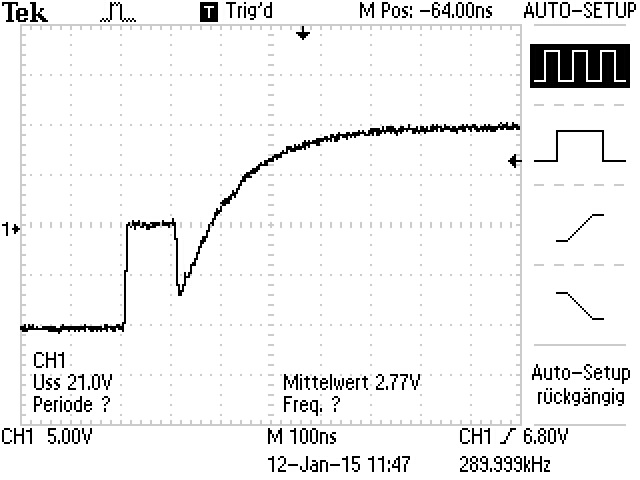
\includegraphics[scale=1.0]{bilder/abschluss/F0005TEK.JPG}
  \caption{Spannungsverlauf mit Abschlusswiderstand 1.}
  \label{fig:abschluss_1}
\end{figure}

\begin{figure}[htpb]
  \centering
  \includegraphics[scale=1.0]{bilder/abschluss_1_fit.pdf}
  \caption{Darstellung der zu Bestimmung der Kapazität linearisierten mit Daten
  mit entsprechenden Fit.}
  \label{fig:abschluss_1_fit}
\end{figure}

\clearpage
\paragraph{Abschluss 4}
\label{ssub:abschluss_4}

Der Spannungsverlauf des Signals mit Abschluss 4 ist in
Abbildung~\ref{fig:abschluss_4} dargestellt. Hierbei handelt es sich um eine
Reihenschaltung von einem Widerstand mit einer Spule.
Die digitalisierten Daten sind in Abbildung~\ref{fig:abschluss_3_digitalisiert}
sowie in Tabelle~\ref{tab:daten_abschluss_4} dargestellt.
Die zur Bestimmung der Widerstandes notwendigen Spannung werden aus
\begin{align}
  \begin{aligned}
    U_\text{off} &= \overline{U(t)}\,, \\
    U_1          &= \overline{U(t)}\,, \\
    U_0          &= \overline{U(t)}\,,
  \end{aligned}
  \qquad
  \begin{aligned}
    \SI{377}{\nano\second}  <~&t~< \SI{455}{\nano\second} \\
    \SI{483}{\nano\second}  <~&t~< \SI{568}{\nano\second} \\
    \SI{2127}{\nano\second}  <~&t~< \SI{2183}{\nano\second}
  \end{aligned}
\end{align}
genommen. Damit ergibt sich für die Spannungen
\begin{align}
  U_\text{off} &= \SI[parse-numbers = false]{14.96 \pm 0.09}{\volt} \\
  U_1 &= \SI[parse-numbers = false]{25.79 \pm 0.14}{\volt} \\
  U_0 &= \SI[parse-numbers = false]{24.36 \pm 0.09}{\volt}
\end{align}
und für den Widerstand
\begin{equation}
  \underline{R = $-40.0$           & $19.2$            & $830.0$           & $142.4$           & $1470.0$          & $62.0$           \\
$5.0$             & $18.4$            & $875.0$           & $142.8$           & $1485.0$          & $58.8$           \\
$40.0$            & $18.0$            & $905.0$           & $143.6$           & $1500.0$          & $54.8$           \\
$90.0$            & $17.6$            & $955.0$           & $144.0$           & $1535.0$          & $53.2$           \\
$130.0$           & $19.2$            & $1015.0$          & $144.0$           & $1560.0$          & $50.0$           \\
$170.0$           & $18.8$            & $1055.0$          & $144.0$           & $1595.0$          & $48.0$           \\
$220.0$           & $18.8$            & $1100.0$          & $144.8$           & $1635.0$          & $47.2$           \\
$255.0$           & $18.4$            & $1150.0$          & $144.4$           & $1675.0$          & $45.6$           \\
$295.0$           & $18.4$            & $1195.0$          & $144.8$           & $1720.0$          & $44.4$           \\
$340.0$           & $18.4$            & $1235.0$          & $145.6$           & $1760.0$          & $44.0$           \\
$385.0$           & $18.0$            & $1280.0$          & $145.6$           & $1800.0$          & $43.6$           \\
$425.0$           & $18.8$            & $1330.0$          & $145.6$           & $1850.0$          & $43.2$           \\
$470.0$           & $18.4$            & $1365.0$          & $146.0$           & $1895.0$          & $43.2$           \\
$510.0$           & $19.2$            & $1370.0$          & $142.0$           & $1945.0$          & $43.2$           \\
$515.0$           & $22.8$            & $1375.0$          & $138.4$           & $1980.0$          & $42.8$           \\
$520.0$           & $30.8$            & $1380.0$          & $130.4$           & $2030.0$          & $42.8$           \\
$525.0$           & $38.4$            & $1385.0$          & $118.8$           & $2075.0$          & $43.2$           \\
$530.0$           & $90.4$            & $1390.0$          & $102.8$           & $2120.0$          & $43.2$           \\
$535.0$           & $106.0$           & $1395.0$          & $99.2$            & $2170.0$          & $43.2$           \\
$540.0$           & $122.0$           & $1400.0$          & $95.2$            & $2215.0$          & $43.2$           \\
$550.0$           & $137.6$           & $1405.0$          & $87.6$            & $2260.0$          & $42.8$           \\
$570.0$           & $139.2$           & $1410.0$          & $83.6$            & $2300.0$          & $42.8$           \\
$605.0$           & $140.8$           & $1415.0$          & $80.0$            & $2345.0$          & $42.0$           \\
$645.0$           & $140.4$           & $1420.0$          & $76.0$            & $2390.0$          & $40.8$           \\
$685.0$           & $141.2$           & $1430.0$          & $72.4$            & $2420.0$          & $40.8$           \\
$730.0$           & $141.6$           & $1440.0$          & $68.8$            & -                 & -                \\
$780.0$           & $142.4$           & $1455.0$          & $65.6$            & -                 & -                \\}~.
\end{equation}
Zur Bestimmung der Induktivität wird ebenso verfahren wie in
Abschnitt~\ref{ssub:bestimmung_der_leitungskonstanten}, wobei die Zeitkonstante
hier
\begin{equation}
  \tau = -\frac{L}{R + Z_0}
\end{equation}
lautet und die Induktivität sich entsprechend
\begin{equation}
  L = - \frac{R + Z_0}{m}
\end{equation}
mit der Steigung $m$ aus der Fitgeraden zusammensetzt.
Für den Fit werden die Werte
\begin{equation}
  \SI{622}{\nano\second} < t < \SI{2135}{\nano\second}
\end{equation}
verwandt, sodass sich die Fitgerade zu
\begin{equation}
  G_L(t) = \SI[parse-numbers = false]{-0.0053 \pm 0.0004}{\per\nano\second}\, \cdot \,t\, + \SI[parse-numbers = false]{11.6 \pm 0.7}{}
\end{equation}
ergibt. Diese ist in Abbildung~\ref{fig:abschluss_4_fit} dargestellt.
Somit ergibt sich schließlich für die Induktivität
\begin{equation}
  \underline{L = \SI[parse-numbers = false]{226.0 \pm 4.2}{\milli\henry}~.}
\end{equation}

\begin{table}[htpb]
  \centering
  \begin{tabular}{cc|cc|cc|cc}
    \midrule
    \midrule
    $t/\si{\nano\second}$ & $U/\si{\volt}$ &
    $t/\si{\nano\second}$ & $U/\si{\volt}$ &
    $t/\si{\nano\second}$ & $U/\si{\volt}$ &
    $t/\si{\nano\second}$ & $U/\si{\volt}$ \\
    \midrule
    \phantom{0}15\phantom{.} & 13.11             & \phantom{0}580\phantom{.} & 32.43             & 1140\phantom{.}   & 29.46             & 1790\phantom{.}   & 25.72            \\
\phantom{0}40\phantom{.} & 13.22             & \phantom{0}595\phantom{.} & 34.74             & 1155\phantom{.}   & 29.56             & 1810\phantom{.}   & 25.42            \\
\phantom{0}60\phantom{.} & 13.32             & \phantom{0}610\phantom{.} & 35.04             & 1170\phantom{.}   & 29.47             & 1830\phantom{.}   & 25.33            \\
\phantom{0}85\phantom{.} & 13.43             & \phantom{0}625\phantom{.} & 35.05             & 1190\phantom{.}   & 29.18             & 1850\phantom{.}   & 25.24            \\
105\phantom{.}    & 13.64             & \phantom{0}645\phantom{.} & 34.86             & 1210\phantom{.}   & 29.18             & 1870\phantom{.}   & 25.45            \\
130\phantom{.}    & 13.55             & \phantom{0}665\phantom{.} & 34.77             & 1225\phantom{.}   & 28.89             & 1890\phantom{.}   & 25.26            \\
150\phantom{.}    & 13.76             & \phantom{0}670\phantom{.} & 34.27             & 1250\phantom{.}   & 28.80             & 1910\phantom{.}   & 25.16            \\
170\phantom{.}    & 13.87             & \phantom{0}690\phantom{.} & 34.08             & 1270\phantom{.}   & 28.61             & 1935\phantom{.}   & 25.07            \\
195\phantom{.}    & 13.88             & \phantom{0}710\phantom{.} & 33.98             & 1290\phantom{.}   & 28.42             & 1950\phantom{.}   & 24.98            \\
215\phantom{.}    & 14.19             & \phantom{0}725\phantom{.} & 33.79             & 1310\phantom{.}   & 28.22             & 1970\phantom{.}   & 24.99            \\
235\phantom{.}    & 14.19             & \phantom{0}740\phantom{.} & 33.50             & 1335\phantom{.}   & 28.13             & 2015\phantom{.}   & 24.81            \\
255\phantom{.}    & 14.40             & \phantom{0}755\phantom{.} & 33.40             & 1355\phantom{.}   & 27.94             & 2040\phantom{.}   & 24.72            \\
280\phantom{.}    & 14.41             & \phantom{0}770\phantom{.} & 33.31             & 1380\phantom{.}   & 27.95             & 2055\phantom{.}   & 24.42            \\
305\phantom{.}    & 14.52             & \phantom{0}790\phantom{.} & 33.12             & 1395\phantom{.}   & 27.66             & 2075\phantom{.}   & 24.63            \\
325\phantom{.}    & 14.53             & \phantom{0}810\phantom{.} & 32.82             & 1420\phantom{.}   & 27.67             & 2095\phantom{.}   & 24.44            \\
345\phantom{.}    & 14.64             & \phantom{0}825\phantom{.} & 32.63             & 1435\phantom{.}   & 27.37             & 2120\phantom{.}   & 24.55            \\
360\phantom{.}    & 14.84             & \phantom{0}850\phantom{.} & 32.44             & 1460\phantom{.}   & 27.38             & 2140\phantom{.}   & 24.36            \\
380\phantom{.}    & 14.95             & \phantom{0}865\phantom{.} & 32.15             & 1480\phantom{.}   & 27.29             & 2155\phantom{.}   & 24.26            \\
405\phantom{.}    & 14.86             & \phantom{0}880\phantom{.} & 32.05             & 1500\phantom{.}   & 27.10             & 2175\phantom{.}   & 24.47            \\
425\phantom{.}    & 15.07             & \phantom{0}900\phantom{.} & 31.86             & 1525\phantom{.}   & 27.11             & 2185\phantom{.}   & 24.07            \\
465\phantom{.}    & 15.79             & \phantom{0}920\phantom{.} & 31.67             & 1540\phantom{.}   & 26.72             & 2190\phantom{.}   & 21.58            \\
470\phantom{.}    & 18.79             & \phantom{0}940\phantom{.} & 31.38             & 1565\phantom{.}   & 26.73             & 2195\phantom{.}   & 18.68            \\
475\phantom{.}    & 21.19             & \phantom{0}955\phantom{.} & 31.18             & 1585\phantom{.}   & 26.53             & 2200\phantom{.}   & 16.18            \\
480\phantom{.}    & 23.69             & \phantom{0}980\phantom{.} & 31.09             & 1605\phantom{.}   & 26.44             & 2205\phantom{.}   & 13.78            \\
485\phantom{.}    & 25.59             & \phantom{0}995\phantom{.} & 30.80             & 1620\phantom{.}   & 26.25             & 2230\phantom{.}   & 13.79            \\
505\phantom{.}    & 25.70             & 1015\phantom{.}   & 30.71             & 1645\phantom{.}   & 26.26             & 2250\phantom{.}   & 13.50            \\
520\phantom{.}    & 25.81             & 1030\phantom{.}   & 30.41             & 1665\phantom{.}   & 26.07             & 2275\phantom{.}   & 13.51            \\
545\phantom{.}    & 25.82             & 1065\phantom{.}   & 30.23             & 1680\phantom{.}   & 26.17             & 2285\phantom{.}   & 13.11            \\
565\phantom{.}    & 26.03             & 1085\phantom{.}   & 30.13             & 1700\phantom{.}   & 25.98             & 2290\phantom{.}   & 11.62            \\
570\phantom{.}    & 28.53             & 1100\phantom{.}   & 29.94             & 1725\phantom{.}   & 25.89             & 2295\phantom{.}   & 10.22            \\
575\phantom{.}    & 30.43             & 1125\phantom{.}   & 29.85             & 1765\phantom{.}   & 25.71             & 2300\phantom{.}   & \phantom{0}8.22  \\
    \midrule
    \midrule
  \end{tabular}
  \caption{Darstellung der digitalisierten Daten.
    Oszillosgraphenbild~\ref{fig:abschluss_4}.}
  \label{tab:daten_abschluss_4}
\end{table}

\begin{figure}[htpb]
  \centering
  \includegraphics[scale=1.0]{bilder/abschluss_4.pdf}
  \caption{Darstellung der digitalisierten Daten aus dem
    Oszillosgraphenbild~\ref{fig:abschluss_4}.}
\label{fig:abschluss_4_digitalisiert}
\end{figure}

\begin{figure}[htpb]
  \centering
  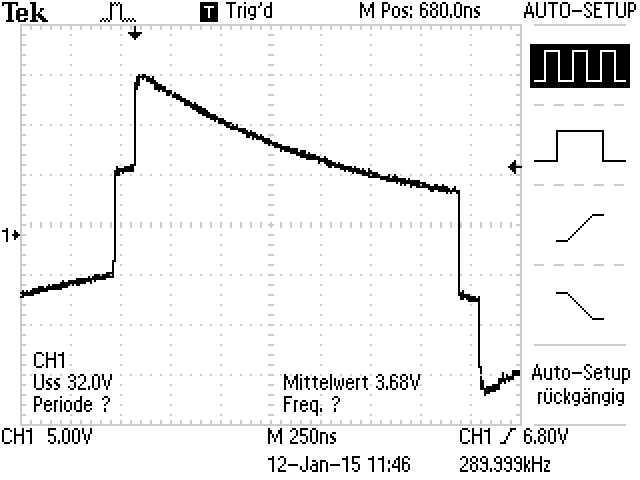
\includegraphics[scale=1.0]{bilder/abschluss/F0004TEK.JPG}
  \caption{Spannungsverlauf mit Abschlusswiderstand 4.}
  \label{fig:abschluss_4}
\end{figure}

\begin{figure}[htpb]
  \centering
  \includegraphics[scale=1.0]{bilder/abschluss_4_fit.pdf}
  \caption{Darstellung der zu Bestimmung der Induktivität
    linearisierten mit Daten mit entsprechenden Fit.}
\label{fig:abschluss_4_fit}
\end{figure}

\clearpage
\paragraph{Abschluss 3}
\label{par:abschluss_3}

Hier befindet sich der Spannungsverlauf in Abbildung~\ref{fig:abschluss_3}.
Der Vergleich mit den Abschlüssen in Abbildung~\ref{fig:abschluesse} liefert
hier einen Abschlusswiderstand, welcher aus einer Parallelschaltung eines
Widerstandes und einem Kondensator besteht.
Zur Berechnung werden die nötigen Spannungen aus
\begin{align}
  \begin{aligned}
    U_\text{off} &= \overline{U(t)}\,, \\
    U_1          &= \overline{U(t)}\,, \\
    U_0          &= \overline{U(t)}\,,
  \end{aligned}
  \qquad
  \begin{aligned}
    &t~< \SI{500}{\nano\second} \\
    \SI{1500}{\nano\second}  <~&t~< \SI{2200}{\nano\second} \\
    \SI{540}{\nano\second}  <~&t~< \SI{607}{\nano\second}
  \end{aligned}
\end{align}
genommen. Diese lauten nach Mittelung
\begin{align}
  U_\text{off} &= \SI[parse-numbers = false]{14.96 \pm 0.09}{\volt} \\
  U_1 &= \SI[parse-numbers = false]{25.79 \pm 0.14}{\volt} \\
  U_0 &= \SI[parse-numbers = false]{24.36 \pm 0.09}{\volt}~.
\end{align}
Daraus ergibt sich der Widerstand zu
\begin{equation}
  \underline{R = $-40.0$           & $19.2$            & $830.0$           & $142.4$           & $1470.0$          & $62.0$           \\
$5.0$             & $18.4$            & $875.0$           & $142.8$           & $1485.0$          & $58.8$           \\
$40.0$            & $18.0$            & $905.0$           & $143.6$           & $1500.0$          & $54.8$           \\
$90.0$            & $17.6$            & $955.0$           & $144.0$           & $1535.0$          & $53.2$           \\
$130.0$           & $19.2$            & $1015.0$          & $144.0$           & $1560.0$          & $50.0$           \\
$170.0$           & $18.8$            & $1055.0$          & $144.0$           & $1595.0$          & $48.0$           \\
$220.0$           & $18.8$            & $1100.0$          & $144.8$           & $1635.0$          & $47.2$           \\
$255.0$           & $18.4$            & $1150.0$          & $144.4$           & $1675.0$          & $45.6$           \\
$295.0$           & $18.4$            & $1195.0$          & $144.8$           & $1720.0$          & $44.4$           \\
$340.0$           & $18.4$            & $1235.0$          & $145.6$           & $1760.0$          & $44.0$           \\
$385.0$           & $18.0$            & $1280.0$          & $145.6$           & $1800.0$          & $43.6$           \\
$425.0$           & $18.8$            & $1330.0$          & $145.6$           & $1850.0$          & $43.2$           \\
$470.0$           & $18.4$            & $1365.0$          & $146.0$           & $1895.0$          & $43.2$           \\
$510.0$           & $19.2$            & $1370.0$          & $142.0$           & $1945.0$          & $43.2$           \\
$515.0$           & $22.8$            & $1375.0$          & $138.4$           & $1980.0$          & $42.8$           \\
$520.0$           & $30.8$            & $1380.0$          & $130.4$           & $2030.0$          & $42.8$           \\
$525.0$           & $38.4$            & $1385.0$          & $118.8$           & $2075.0$          & $43.2$           \\
$530.0$           & $90.4$            & $1390.0$          & $102.8$           & $2120.0$          & $43.2$           \\
$535.0$           & $106.0$           & $1395.0$          & $99.2$            & $2170.0$          & $43.2$           \\
$540.0$           & $122.0$           & $1400.0$          & $95.2$            & $2215.0$          & $43.2$           \\
$550.0$           & $137.6$           & $1405.0$          & $87.6$            & $2260.0$          & $42.8$           \\
$570.0$           & $139.2$           & $1410.0$          & $83.6$            & $2300.0$          & $42.8$           \\
$605.0$           & $140.8$           & $1415.0$          & $80.0$            & $2345.0$          & $42.0$           \\
$645.0$           & $140.4$           & $1420.0$          & $76.0$            & $2390.0$          & $40.8$           \\
$685.0$           & $141.2$           & $1430.0$          & $72.4$            & $2420.0$          & $40.8$           \\
$730.0$           & $141.6$           & $1440.0$          & $68.8$            & -                 & -                \\
$780.0$           & $142.4$           & $1455.0$          & $65.6$            & -                 & -                \\}~.
\end{equation}
Die Kapazität wird wieder über eine Linearisierung bestimmt, wobei die Werte aus
\begin{equation}
  \SI{1500}{\nano\second} < t < \SI{2000}{\nano\second}
\end{equation}
genommen werden. Die Sättigungsspannung entspricht $U_1$.
Der Fit ergibt die Gerade
\begin{equation}
  1375\phantom{.}   & 215.910           & 95.869            & 4.563            \\
1380\phantom{.}   & 225.883           & 85.896            & 4.453            \\
1385\phantom{.}   & 234.859           & 76.920            & 4.343            \\
1390\phantom{.}   & 244.832           & 66.947            & 4.204            \\
1395\phantom{.}   & 253.807           & 57.972            & 4.060            \\
1405\phantom{.}   & 262.781           & 48.998            & 3.892            \\
1420\phantom{.}   & 271.753           & 40.026            & 3.690            \\
1435\phantom{.}   & 279.727           & 32.052            & 3.467            \\
1465\phantom{.}   & 286.697           & 25.082            & 3.222            \\
1490\phantom{.}   & 292.672           & 19.107            & 2.950            \\
1525\phantom{.}   & 296.648           & 15.131            & 2.717            \\
1560\phantom{.}   & 301.622           & 10.157            & 2.318            \\
1600\phantom{.}   & 303.601           & \phantom{0}8.178  & 2.101            \\
1645\phantom{.}   & 305.578           & \phantom{0}6.201  & 1.825            \\~.
\end{equation}
In der Parallelschaltung ergibt sich die Zeitkonstante zu
\begin{equation}
  \tau = \qty(\frac{1}{Z_0} + \frac{1}{R}) C~,
\end{equation}
sodass sich die Kapazität aus der Steigung der Fitgeraden gemäß
\begin{equation}
  C = \frac{1}{m \qty(\frac{1}{Z_0} + \frac{1}{R})}
\end{equation}
bestimmen lässt und sich schließlich zu
\begin{equation}
  \underline{C = \SI[parse-numbers = false]{1.82 \pm 0.16}{\nano\farad}}
\end{equation}
ergibt.
Der Fit ist dabei in Abbildung~\ref{fig:abschluss_3_fit} dargestellt.

\begin{table}[htpb]
  \centering
  \begin{tabular}{cc|cc|cc|cc}
    \midrule
    \midrule
    $t/\si{\nano\second}$ & $U/\si{\volt}$ &
    $t/\si{\nano\second}$ & $U/\si{\volt}$ &
    $t/\si{\nano\second}$ & $U/\si{\volt}$ &
    $t/\si{\nano\second}$ & $U/\si{\volt}$ \\
    \midrule
    \phantom{0}15\phantom{.} & 14.71             & \phantom{0}620\phantom{.} & 22.25             & 1085\phantom{.}   & 27.84             & 1815\phantom{.}   & 27.94            \\
\phantom{0}40\phantom{.} & 14.71             & \phantom{0}625\phantom{.} & 20.39             & 1105\phantom{.}   & 27.75             & 1840\phantom{.}   & 27.94            \\
\phantom{0}50\phantom{.} & 14.41             & \phantom{0}630\phantom{.} & 18.92             & 1125\phantom{.}   & 27.75             & 1865\phantom{.}   & 27.94            \\
\phantom{0}60\phantom{.} & 14.71             & \phantom{0}645\phantom{.} & 18.14             & 1145\phantom{.}   & 27.84             & 1880\phantom{.}   & 28.14            \\
\phantom{0}80\phantom{.} & 14.80             & \phantom{0}650\phantom{.} & 18.63             & 1170\phantom{.}   & 27.94             & 1900\phantom{.}   & 27.94            \\
105\phantom{.}    & 15.00             & \phantom{0}660\phantom{.} & 19.02             & 1190\phantom{.}   & 27.94             & 1920\phantom{.}   & 28.14            \\
120\phantom{.}    & 14.80             & \phantom{0}665\phantom{.} & 19.41             & 1210\phantom{.}   & 27.84             & 1945\phantom{.}   & 27.94            \\
145\phantom{.}    & 14.80             & \phantom{0}670\phantom{.} & 19.90             & 1230\phantom{.}   & 27.84             & 1965\phantom{.}   & 27.94            \\
165\phantom{.}    & 14.90             & \phantom{0}680\phantom{.} & 20.29             & 1255\phantom{.}   & 27.94             & 1985\phantom{.}   & 28.04            \\
185\phantom{.}    & 14.90             & \phantom{0}685\phantom{.} & 20.69             & 1275\phantom{.}   & 27.75             & 1995\phantom{.}   & 27.75            \\
215\phantom{.}    & 14.90             & \phantom{0}690\phantom{.} & 21.18             & 1295\phantom{.}   & 28.04             & 2015\phantom{.}   & 27.84            \\
235\phantom{.}    & 14.71             & \phantom{0}700\phantom{.} & 21.57             & 1310\phantom{.}   & 27.94             & 2040\phantom{.}   & 27.94            \\
265\phantom{.}    & 14.80             & \phantom{0}705\phantom{.} & 21.96             & 1335\phantom{.}   & 28.04             & 2055\phantom{.}   & 27.84            \\
275\phantom{.}    & 15.00             & \phantom{0}725\phantom{.} & 22.25             & 1360\phantom{.}   & 27.94             & 2080\phantom{.}   & 27.94            \\
315\phantom{.}    & 14.80             & \phantom{0}730\phantom{.} & 22.75             & 1380\phantom{.}   & 28.04             & 2105\phantom{.}   & 27.84            \\
340\phantom{.}    & 14.80             & \phantom{0}745\phantom{.} & 22.94             & 1400\phantom{.}   & 27.84             & 2130\phantom{.}   & 27.94            \\
365\phantom{.}    & 14.61             & \phantom{0}765\phantom{.} & 23.92             & 1425\phantom{.}   & 28.04             & 2155\phantom{.}   & 27.94            \\
380\phantom{.}    & 14.90             & \phantom{0}775\phantom{.} & 24.31             & 1445\phantom{.}   & 27.94             & 2175\phantom{.}   & 28.04            \\
415\phantom{.}    & 14.90             & \phantom{0}785\phantom{.} & 24.71             & 1470\phantom{.}   & 27.94             & 2200\phantom{.}   & 27.84            \\
440\phantom{.}    & 14.71             & \phantom{0}800\phantom{.} & 25.00             & 1495\phantom{.}   & 28.04             & 2225\phantom{.}   & 27.94            \\
465\phantom{.}    & 14.80             & \phantom{0}815\phantom{.} & 25.29             & 1515\phantom{.}   & 27.84             & 2235\phantom{.}   & 27.65            \\
490\phantom{.}    & 14.90             & \phantom{0}825\phantom{.} & 25.69             & 1535\phantom{.}   & 28.04             & 2240\phantom{.}   & 25.20            \\
505\phantom{.}    & 15.00             & \phantom{0}845\phantom{.} & 25.69             & 1555\phantom{.}   & 28.04             & 2245\phantom{.}   & 22.84            \\
510\phantom{.}    & 16.47             & \phantom{0}855\phantom{.} & 26.08             & 1575\phantom{.}   & 28.04             & 2250\phantom{.}   & 20.39            \\
515\phantom{.}    & 17.84             & \phantom{0}875\phantom{.} & 26.37             & 1595\phantom{.}   & 28.04             & 2255\phantom{.}   & 18.04            \\
520\phantom{.}    & 20.29             & \phantom{0}890\phantom{.} & 26.67             & 1620\phantom{.}   & 27.94             & 2270\phantom{.}   & 17.75            \\
525\phantom{.}    & 23.14             & \phantom{0}915\phantom{.} & 26.76             & 1635\phantom{.}   & 27.84             & 2295\phantom{.}   & 17.84            \\
530\phantom{.}    & 24.12             & \phantom{0}935\phantom{.} & 26.96             & 1660\phantom{.}   & 28.04             & 2320\phantom{.}   & 17.75            \\
540\phantom{.}    & 24.90             & \phantom{0}955\phantom{.} & 27.06             & 1680\phantom{.}   & 28.04             & 2335\phantom{.}   & 17.84            \\
565\phantom{.}    & 24.90             & \phantom{0}970\phantom{.} & 27.25             & 1705\phantom{.}   & 27.94             & 2340\phantom{.}   & 19.80            \\
585\phantom{.}    & 25.10             & 1015\phantom{.}   & 27.55             & 1725\phantom{.}   & 27.94             & 2345\phantom{.}   & 21.18            \\
605\phantom{.}    & 25.10             & 1035\phantom{.}   & 27.45             & 1745\phantom{.}   & 27.94             & 2350\phantom{.}   & 23.14            \\
610\phantom{.}    & 24.61             & 1050\phantom{.}   & 27.65             & 1770\phantom{.}   & 27.94             & -                 & -                \\
615\phantom{.}    & 24.22             & 1070\phantom{.}   & 27.55             & 1795\phantom{.}   & 27.84             & -                 & -                \\
    \midrule
    \midrule
  \end{tabular}
  \caption{Darstellung der digitalisierten Daten.
    Oszillosgraphenbild~\ref{fig:abschluss_3}.}
  \label{tab:daten_abschluss_3}
\end{table}

\begin{figure}[htpb]
  \centering
  \includegraphics[scale=1.0]{bilder/abschluss_3.pdf}
  \caption{Darstellung der digitalisierten Daten aus dem
    Oszillosgraphenbild~\ref{fig:abschluss_3}.}
\label{fig:abschluss_3_digitalisiert}
\end{figure}

\begin{figure}[htpb]
  \centering
  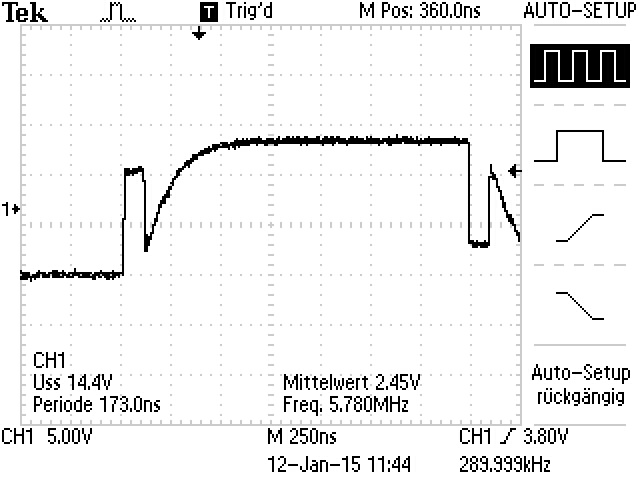
\includegraphics[scale=1.0]{bilder/abschluss/F0003TEK.JPG}
  \caption{Spannungsverlauf mit Abschlusswiderstand 3.}
  \label{fig:abschluss_3}
\end{figure}

\begin{figure}[htpb]
  \centering
  \includegraphics[scale=1.0]{bilder/abschluss_3_fit.pdf}
  \caption{Darstellung der zu Bestimmung der Induktivität
    linearisierten mit Daten mit entsprechenden Fit.}
\label{fig:abschluss_3_fit}
\end{figure}

